\chapter{Experimentos y evaluación}
\label{cap:experimentos}

\section{Implementación del sistema}
%Acá hay que hablar de todo lo que implementaste a grandes rasgos (detalles Anexo), modelo, manejo de réplicas, etc. Redactar de nuevo

Para la implementanción del sistema propuesto, se utilizó como base el motor de procesamiento de \textit{stream} S4 \citep{s4}, cuyo modelo fue explicado en la sección \ref{sec:SPS}. El funcionamiento del sistema de distribución de carga propuesto se desarrolló en Java, donde se modificó en el código fuente de S4, para incluir las funciones de este producto, de tal manera que fuera automático y transparente para el usuario del SPS.

El sistema diseñado fue añadido al proyecto S4, siendo una paquete denominado \textit{monitor} que contenía las clases \textit{S4Monitor}, \textit{MarkovChain}, \textit{MonitorMetrics}, \textit{StatusPE} y \textit{TopologyApp}. La primer clase correspondía a las funcionalidades del sistema de monitoreo, ya sea la recepción de los datos del sistema, ejecución del algoritmo reactivo o predictivo y administración de las réplicas de cada operador. La segunda clase hacía alusión al modelo de cadena de Markov implementando por el algoritmo predictivo, donde posee tanto la conformación de la matriz de transición como el cálculo de la distribución estacionaria. La tercera clase se utilizó para recolectar las estadísticas de cada operador, y poder analizar los experimentos. Finalmente, la cuarta y quinta clase fueron utilizadas para la implementación del sistema de monitoreo, siendo la primera el estado de cada PE y el segundo la topología que poseía el grafo creado por el usuario, los cuales pueden verse con más detalle en el Anexo \ref{apendice:clases}.

Para la ejecución del SPS conjunto con el monitor, se debe en primer lugar registrar los PEs. Para esto, se implementó una función que tenga como parámetro dos PEs, donde el primero es el PE emisor y el segundo el receptor. Esta información es importante para obtener la topología del grafo, dado que con esto se puede realizar un análisis del rendimiento de los PEs.

Además de lo anterior, para el análisis de cada uno de los PEs, se añadió los atributos de cantidad de eventos entrantes y salientes cada un segundo y cinco segundos en la clase del PE. Esto fue utilizado posteriormente para las estadísticas deseadas para el algoritmo reactivo y predictivo. La tasa de llegada es considerada desde el momento que se recibe el evento desde el PE emisor, y la tasa de servicio es considera desde el momento que se termina de realizar la ejecución de la tarea en el PE. Además, se agregó un atributo booleano, el cual indica si el PE puede aumentar o disminuir la cantidad de réplicas que posee al iniciar el sistema.

Posteriormente, para el funcionamiento del sistema de distribución de carga se procedió a ejecutar dos tareas en la aplicación de S4: una tarea que guarde las muestras para el historial del operador y otra que envíe las estadísticas del operador, las cuales poseían un intervalo de ejecución de 1 y 5 segundos respectivamente. La primera tarea analiza cada uno de los PEs, tomando en consideración las estadísticas de eventos entrantes y salientes, los cuales darán origen a la tasa de llegada ($\lambda$) y servicio ($\mu$), para que posteriormente se calcule la tasa de rendimiento en la ventana de tiempo analizada, guardando así la muestra en el historial. La segunda tarea obtiene las estadísticas de cada uno de los PEs, ya sea la tasa de llegada ($\lambda$) y servicio ($\mu$), dado los eventos entrantes y saliente, cantidad de eventos totales e historial del PE, los cuales son enviados al monitoreo de carga, para posteriormente ejecutar el algoritmo que corresponda según la ventana de tiempo, y finalmente realizar la administración de réplicas para aumentar o disminuir las réplicas necesarias en cada operador según lo necesario. El código de la implementanción se puede observar en el Anexo \ref{apendice:codigoFuenteS4}.

Debido al funcionamiento de los SPS, existe una fuente de datos, por lo tanto, para la correcta sincronización de las estadísticas, se procedió a realizar una espera por parte del monitor hasta que la fuente de datos esté lista para enviar los datos. Esta implementanción se puede ver en el Anexo \ref{apendice:codigoFuenteS4}, conjunto con las dos tareas que debe ejecutar después que la fuente de datos avisa de su inicialización.

En el caso del envío de las estadísticas, después de ser enviadas, se consulta el estado de cada uno de los operadores, y en caso de ser necesario, se realiza las modificaciones necesarias en el sistema, ya sea de crear o eliminar réplicas de un operador. En el caso de crear réplicas, lo que se realiza es consultar la cantidad de réplicas que dijo que deben existir por parte del administrador de réplicas, y en caso de poseer un número de réplicas mayor que el existente por el PE, se procede a crear la cantidad de réplicas faltantes. Por otra parte, en caso de que el número sea menor, procede a terminar la ejecución del PE y posteriormente elimina la cantidad de réplicas sobrantes. En caso que el operador que se haya identificado con el atributo único, significa que no puede aumentar ni disminuir la cantidad de réplicas asignadas a éste. Los códigos de crear o eliminar replicas se encuentra adjuntos en el Anexo \ref{apendice:codigoFuenteS4}.

Dado que en el diseño se propuso un mecanismo de balance de carga basado en la técnica de replicación, fue necesario modificar S4, de manera de poder manejar las réplicas para los operadores. Se implementó el SPS de tal manera de poder manejar un algoritmo que escogiera la réplica que tuviera menor tamaño en la cola de espera al momento de enviar un dato, y así siempre escoger al operador con menor carga, y en caso que posean el mismo tamaño, utilizar la primera réplica disponible.

En la Figura \ref{fig:distCarga} se explica gráficamente la distribución de la carga. En la parte (a) el operador A envía un evento al operador B, el cual posee tres réplicas, cuyas menores colas están en la réplica 2 y 3, como son iguales las colas de estas réplicas, se escoge la primera réplica disponible, es decir, la réplica 2. Posteriormente, como la réplica 2 aumento su cola, la réplica 3 es la que posee menor cantidad de cola, como se demuestra en la parte (b), por lo tanto, es la réplica candidata a recibir el dato enviado. Y finalmente, en la parte (c) todas las réplicas posee el mismo tamaño de la cola, por lo tanto, se procede a enviar a la primera réplica.

\begin{figure}[!ht]
	\centering
		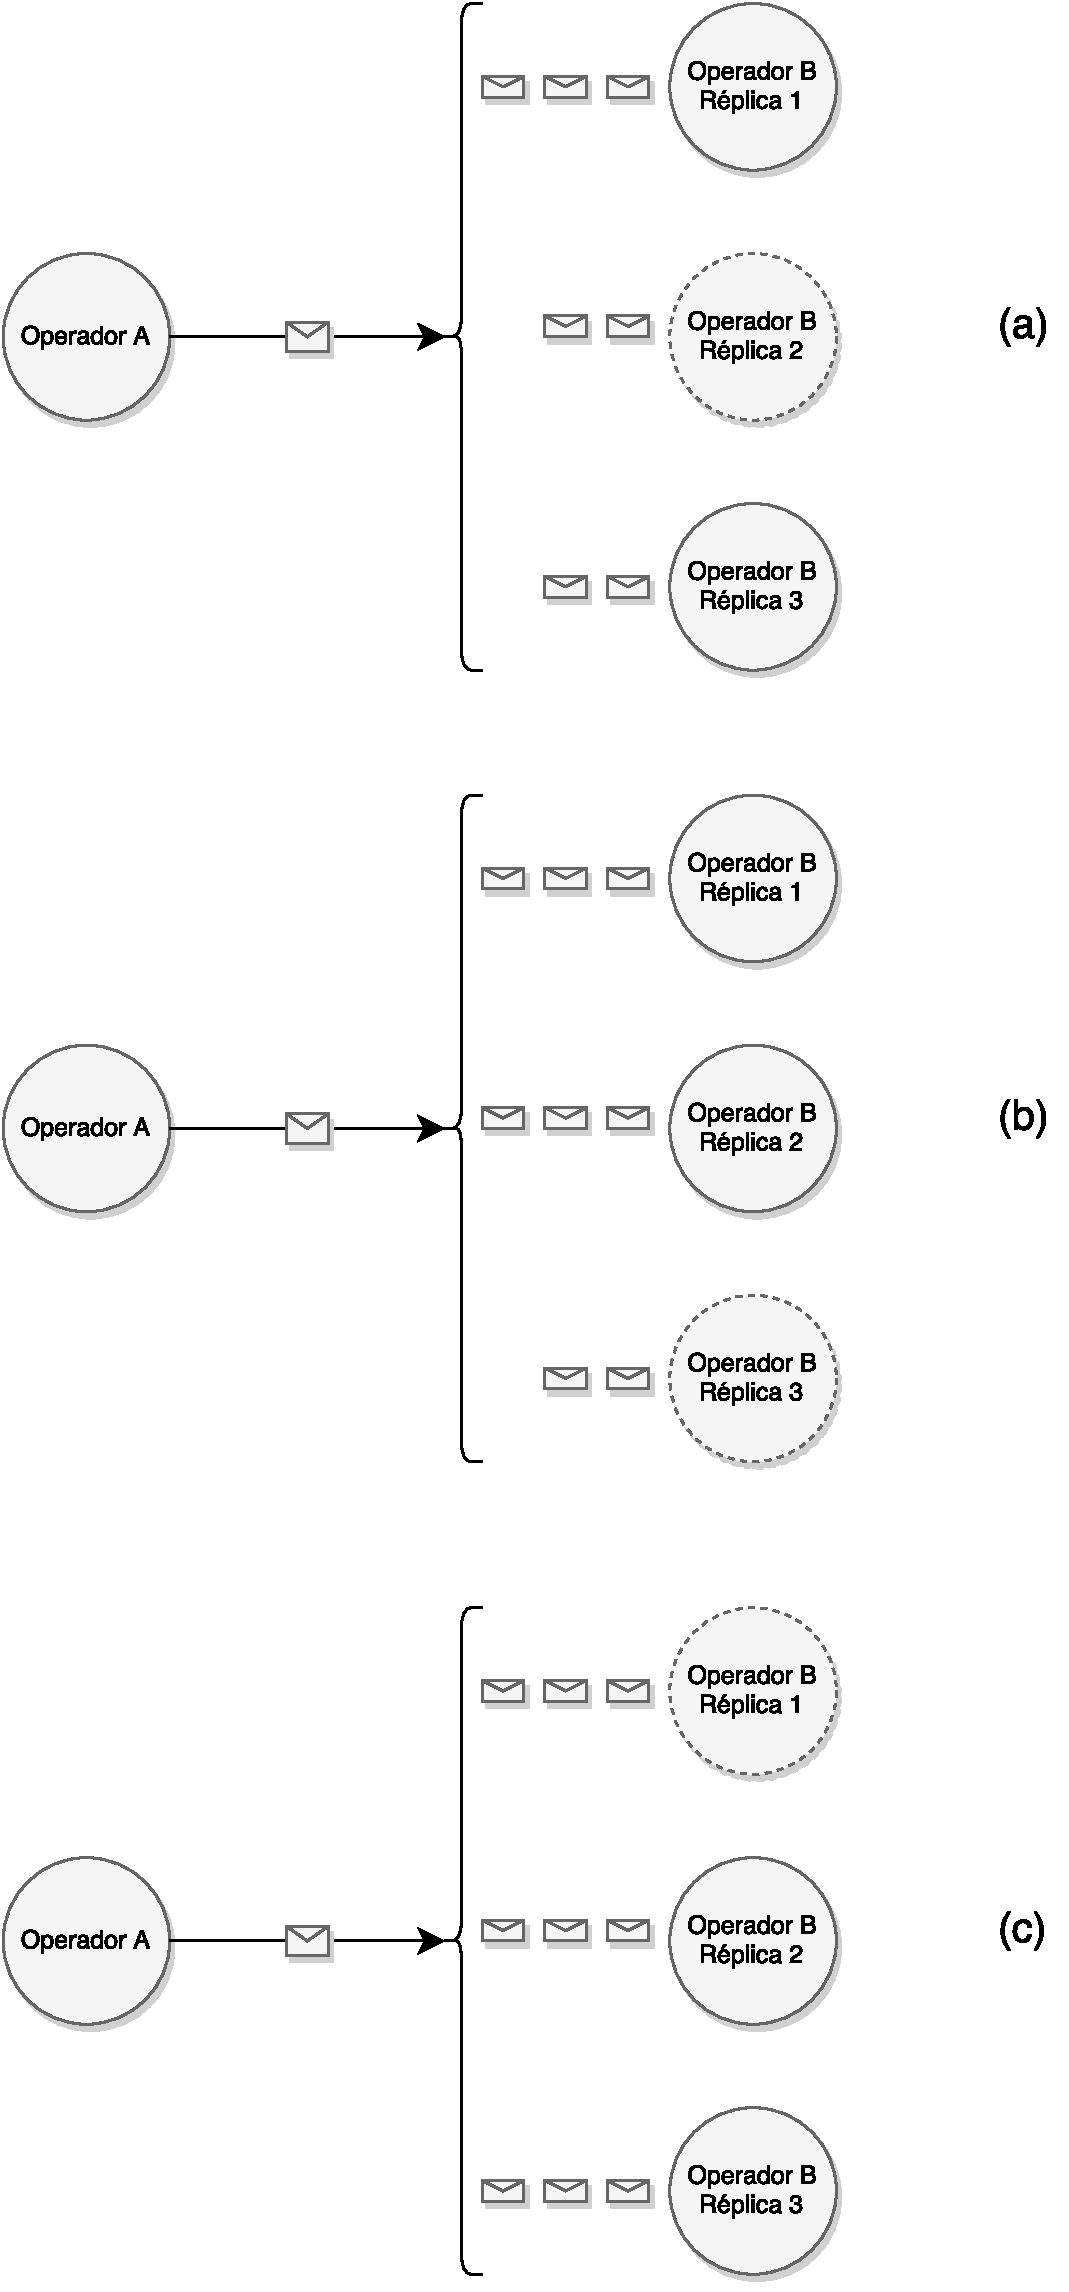
\includegraphics[scale=0.55]{images/DistribucionCarga.pdf}
	\caption{Distribución de la carga entre las réplicas.}
	\label{fig:distCarga}
\end{figure}

En el Algoritmo \ref{alg:distCarga} está descrito la distribución de carga planteada anteriormente, la cual fue implementada en S4 para realizar los experimentos según lo diseñado en el planteamiento de los algoritmos.

\begin{algorithm}[!ht]
	\caption{Distribución de carga entre las réplicas de un operador.}
	\label{alg:distCarga}
	\begin{algorithmic}[1]
	\REQUIRE Evento $\epsilon$ y operador $\phi$.
	\ENSURE Envío del evento a la réplica disponible del operador $\phi$.
	\STATE $\theta \leftarrow minTamanoCola(\phi)$ \COMMENT Se escoge la réplica que posea menor cola
	\STATE $envioEvento(\epsilon,\theta$)
	\end{algorithmic}
\end{algorithm}

\section{Diseño de los experimentos}
Para los experimentos se diseñaron tres aplicaciones, una que realiza operaciones con estado, otra que no, y otra que es sintética. En el caso que la aplicación posea estado, significa que el operador guarda variables con el transcurso del tiempo, las cuales van a ser entregadas cada cierto tiempo o al finalizar la ejecución del sistema. Un ejemplo de esto, es un sistema que cuenta las palabras de un texto y que envié la cantidad de palabras contadas cada cierta ventana de tiempo. Por otra parte, la aplicación sintética se refiere a un sistema cuyos operadores sólo generan tiempo de demora artificial, en el caso de este experimento, se dejo durmiendo la hebra asignada al operador un período determinado de tiempo.

Para la generación del \textit{stream} de la fuente de datos para la primera y segunda aplicación, se utilizaron datos de muestra utilizados fueron \textit{tweets} recolectados entre los días 27 y 28 de Febrero y 1 y 2 de Marzo de 2010, tanto en inglés, portugués y español, cuya información correspondía a la interacción entre los usuarios debido al terremoto ocurrido el 27 de Febrero en el territorio Chile.

Por otra parte, el envío de los datos anteriores se realizó de dos maneras: constante y variable. La primera forma consiste en enviar 100 eventos por segundo constantemente. En cambio, la segunda forma consiste en enviar 50 eventos por segundos el primer tercio del experimento, para luego aumentar a 75 eventos por segundo, los primeros 120 segundos del segundo tercio, y seguir aumentando a 100 eventos por segundo, para posteriormente volver a 75 eventos por segundos los últimos 120 segundos del segundo tercio, y finalmente, disminuir a 50 eventos por segundos el último tercio de la ejecución.

%Estos datos fueron enviados de dos formas: el primero de forma uniforme, enviado 100 eventos por segundos constantemente, y la segundo de forma variable, enviado 50 eventos por segundo el primer tercio de la ejecución del programa, para posteriormente aumentarla a 100 eventos por segundo en el segundo tercio, y finalmente disminuirla a 50 eventos por segundo en el último tercio de la ejecución del programa.

\subsection{Análisis de \textit{tweets} en escenarios de desastres naturales}
La primera aplicación fue orientada a un caso de desastres naturales, donde se generó un grafo que pudiera realizar un filtrado de palabras y análisis de los datos. Ninguno de los operadores posee estado, por lo tanto son independientes. Para la duración de esta prueba se consideró un tiempo de 70 minutos.

La aplicación consta del flujo de datos, cuyos datos serán la muestra de \textit{tweets} de prueba, y cuatro operadores, los cual son denominados \textit{Stopword}, \textit{Language}, \textit{Counter} y \textit{MongoDB}.

\paragraph{Stopword}: está encargado de analizar el \textit{tweet} y remover las palabras no relevantes para el análisis de éste, basado en una bolsa de palabras, cuyas palabras se llaman \textit{stopwords}. De esta manera, se puede analizar el texto usando las palabras más representativas de éste y así entregar información más precisa.

\paragraph{Language}: está encargado de analizar el lenguaje existente en el \textit{tweet}, para esto se utilizó una librería \textit{Apache Tika} \citep{mattmann2011tika}. Con ésta se puede realizar un filtro del idioma de los tweets, de tal manera que en caso de ser requerido, sólo continúen los de un idioma en específico, en nuestro caso el español.

\paragraph{Counter}: está encargado de contar e indicar la cantidad de palabras que existen en el \textit{tweet} según una bolsa de palabras proporcionada por el programador. Para esta prueba se utilizó una bolsa de 26.000 palabras en español. Con esto se podría realizar un análisis de los \textit{tweets} que poseían mayor cantidad de palabras claves asociados a una temática o evento en particular.

\paragraph{MongoDB}: está encargado de guardar en la base de datos el evento según los atributos que éste posea, ya sea por el \textit{tweet} original, sin \textit{stopword}, idioma y cantidad de palabras claves existentes en él. Para esto, se utilizó el motor de base de datos no relacional \textit{MongoDB} \citep{chodorow2013mongodb}.

En la Figura \ref{fig:primeraAplicacion} se muestra un ejemplo de la aplicación con sus distintos operadores y relaciones. Las flechas muestran la dirección del flujo de datos emitido por la fuente y los operadores.

\begin{figure}[!hb]
	\centering
		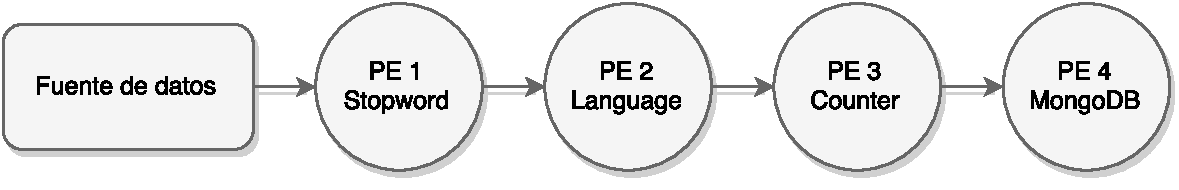
\includegraphics[scale=0.75]{images/App1.pdf}
	\caption{Primera aplicación de prueba.}
	\label{fig:primeraAplicacion}
\end{figure}

\subsection{Contador de palabras en muestras de textos}
La segunda aplicación consiste en un contador de palabras, el cual cuenta la cantidad de veces que se repite una palabra en un conjunto de datos según una bolsa de palabras establecida por el usuario. Esta aplicación se considera con estado, debido que debe existir un contador en el operador, de tal manera de contar la cantidad de veces que se repite cierta palabra de la bolsa de palabras en los datos entrantes. Con esta aplicación es posible analizar posteriormente las palabras más frecuentes emitidas por los usuarios de la red social según un listado de palabras claves. Para la duración de esta prueba se consideró un tiempo de 70 minutos.

La aplicación consta del flujo de datos, cuyos datos serán la muestra de \textit{tweets} de prueba, y tres operadores, denominados \textit{Split}, \textit{Counter} y \textit{Merge}.

\paragraph{Split}: está encargado de dividir el \textit{tweet}, y enviar un arreglo con las palabras que poseía este texto al operador \textit{Counter}.

\paragraph{Counter}: está encargado de guardar las estadísticas de los contadores de cada palabra, es decir, en el momento que reciba un evento, este analiza las palabras que posee y aumenta el contar de la palabra en el operador. Las estadísticas son enviadas cada 10 segundos al operador Merge, de tal manera de no enviar flujo constante al siguiente operador y generar mayor cantidad de carga.

\paragraph{Merge}: está encargado de unir las distintas estadísticas enviadas por las distintas réplicas del operador Counter.

En la Figura \ref{fig:segundaAplicacion} se muestra un ejemplo de la segunda aplicación con sus distintos operadores y sus relaciones, de igual manera que en el caso anterior, las flechas reflejan el flujo de datos. Cabe destacar que el único operador que puede replicarse es el \textit{Counter}, debido que el operador \textit{Split} y \textit{Merge} son operadores que soportan la replicación del operador \textit{Counter}, como se explicó en las técnicas de balance de carga en la subsección \ref{sec:fisionBC}.

\begin{figure}[!hb]
	\centering
		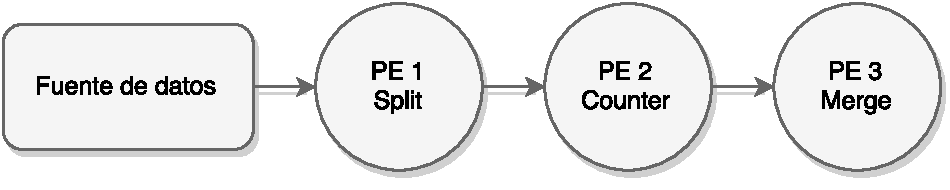
\includegraphics[scale=0.75]{images/App2.pdf}
	\caption{Segunda aplicación de prueba.}
	\label{fig:segundaAplicacion}
\end{figure}

\subsection{Aplicación sintética}
La tercera aplicación consta de tres operadores, los cuales duermen a la hebra asignada al operador un determinado período de tiempo. De esta manera, se genera un tiempo de espera artificial, realizando un operador sintético, de tal manera que pueda simular el comportamiento de un operador real.

La tabla \ref{tab:app3-time} muestra el período de tiempo que duerme cada PEs a su hebra asignada. Los tiempos que se consideraron para esta prueba es para generar una sobrecarga en el primer y segundo operador, de tal manera que después afectarán al tercer operador. Para la duración de esta prueba se consideró un tiempo de 15 minutos.

\begin{table}[!ht]
\centering
\begin{tabular}{| c | c |}
\hline
PE & Tiempo (ms) \\ \hline
1 & 20 \\
2 & 30 \\
3 & 15 \\\hline
\end{tabular}
\caption{Período de tiempo que duerme la hebra asignada al PE.}
\label{tab:app3-time}
\end{table}

En la Figura \ref{fig:terceraAplicacion} se muestra un ejemplo de la tercera aplicación con sus distintos operadores y sus relaciones, de igual manera que en los casos anteriores, las flechas reflejan el flujo de datos.

\begin{figure}[!hb]
	\centering
		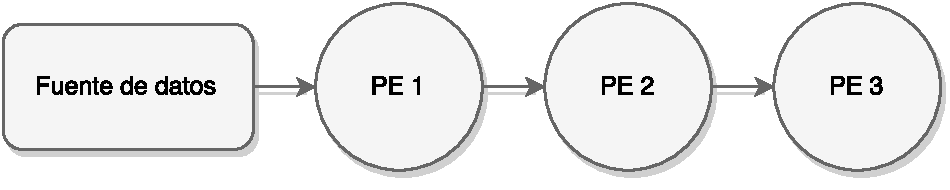
\includegraphics[scale=0.75]{images/App3.pdf}
	\caption{Tercera aplicación de prueba.}
	\label{fig:terceraAplicacion}
\end{figure}

\section{Evaluación}

Para la ejecución de los experimentos, se utilizó un servidor con sistema operativo Ubuntu 14.04.2 LTS, cuyo procesador es un Intel\textregistered Xeon\textregistered CPU E5-2650 v2 de 2.60GHz y con 32 GB de RAM. Cabe recalcar, que el lenguaje de programación fue Java, debido a la integración del sistema propuesto en el SPS utilizado, el cual fue S4. La configuración de la configuración de S4 está detallada en el Anexo \ref{apendice:config-comm-S4}.

La recolección de estadísticas fue realizada cada 5 segundos, por lo que desde ahora se hablará período un intervalo de tiempo de 5 segundos entre cada recolección de las estadísticas.

\subsection{Primera aplicación}
En la primera aplicación se procedió a realizar cuatro experimentos, donde cada par era una comparación del experimento con y sin uso del monitor. Las dos primeras se utilizó flujo constante de la fuente de datos, y las dos segundas un flujo dinámico de la fuente de datos.

Para el análisis de los experimento se consideró la cantidad promedio de eventos procesados en un período, la cantidad total de eventos procesados y las estadísticas de cada PE en el transcurso de la ejecución de la aplicación.

Para analizar el comportamiento del sistema en el primer y segundo experimento, se procedió a estudiar las estadísticas de cada uno de los PEs. En la Figura \ref{fig:app1-uniform-statusStopwordPE-cm} y \ref{fig:app1-uniform-statusStopwordPE-sm} se muestran las estadísticas del primer operador del grafo, con y sin monitoreo en la carga de los operadores respectivamente. En la tasa de llegada ($\lambda$) se puede observar como en el primer gráfico es constante, pero no así en el segundo gráfico, debido que en el segundo 2600 surge una disminución del flujo de datos. Esto se debe a la acumulación de eventos en el \textit{buffer}, por lo que se genera cola en el PE, lo cual impide almacenar mayor cantidad de eventos, dado que la cantidad de eventos que se procesan es menor que la cantidad de eventos que llegan. Por lo tanto, al llenarse el \textit{buffer}, no puede seguir almacenando eventos en la cola, siendo éste bloqueado, habiendo una cola constante como se puede apreciar.

Por otra parte, la tasa de rendimiento de la Figura \ref{fig:app1-uniform-statusStopwordPE-cm} se estabiliza dentro de los primeros 100 segundos, debido que el sistema de distribución de carga detectó una sobrecarga en el operador y replicó el operador, a diferencia de la Figura \ref{fig:app1-uniform-statusStopwordPE-sm}, en el cual el operador posee una tasa de rendimiento estable que bordea entre 1 y 2, hasta el segundo 2600, donde disminuye debido que la tasa de llegada es menor. Cabe destacar que en este operador se encontró una sobrecarga, debido que posee un alto costo computacional, debido que existe una gran cantidad de palabras que debe analizar con cada una de las palabras del texto, por lo que se hace necesario otra réplica en el sistema.

En la Figura \ref{fig:app1-uniform-statusLanguagePE-cm} y \ref{fig:app1-uniform-statusLanguagePE-sm} se puede ver el siguiente operador del gráfico, el cual no tiene mayor inconveniente, a excepción del segundo 2400, donde el sin monitoreo disminuye considerablemente la tasa de procesamiento del PE. Si analizamos la Figura \ref{fig:app1-uniform-statusStopwordPE-sm} y \ref{fig:app1-uniform-statusLanguagePE-sm}, empiezan aproximadamente desde el rango de tiempo (2400s,2600s) los problemas de procesamiento de los operadores, por lo tanto, se puede deducir que si el problema surge en un operador no es un problema aislado, sino que también influye a los siguientes operadores.

Se puede observar como con el transcurso de los primeros 100 segundos en la Figura \ref{fig:app1-uniform-statusCounterPE-cm}, fue aumentando la cantidad de réplicas hasta llegar a 5, el cual fue su óptimo, para ir procesando la cantidad de eventos y disminuir la cola existente en el sistema. Esto en contra posición a la Figura \ref{fig:app1-uniform-statusCounterPE-sm}, donde la inexistencia de replicación, genera una cola la cual se mantiene constante en el segundo 2400. 

Finalmente, se encuentra el último operador, el cual no presenta grandes inconvenientes tanto en la Figura \ref{fig:app1-uniform-statusMongoPE-cm} y \ref{fig:app1-uniform-statusMongoPE-sm}, esto debido que el tiempo de procesamiento es bajo, y nunca llega una cantidad de eventos considerable para existir una sobrecarga en éste. Además es importante destacar que en la Figura \ref{fig:app1-uniform-statusMongoPE-sm} llega una menor tasa de llegada, exactamente un $83,827\%$ menos de eventos que un SPS ejecutado con el sistema de distribución de carga.

Por otra parte, también se analizó la cantidad promedio de eventos procesados en cada período, la cual está graficada en la Figura \ref{fig:app1-uniform-cm-avgEventProcess} y \ref{fig:app1-uniform-sm-avgEventProcess}. Como se puede apreciar, en los primeros 50 segundos se puede ver una mejora considerable en la cantidad de eventos procesados, donde posteriormente se procesan aproximadamente 480 eventos por período con monitoreo, a diferencia del SPS sin monitoreo, que procesa 90 eventos por período aproximadamente, habiendo una mejora del $615,38\%$. Esta mejora se debe al factor de la replicación de los operadores que posee mayor sobrecarga, por lo que al aumentar la cantidad de réplicas, aumenta la tasa de procesamiento, lo significa mayor cantidad de flujo para el próximo operador.

Así también, se puede observar en la Figura \ref{fig:app1-uniform-eventCount-cm} y \ref{fig:app1-uniform-eventCount-sm} la cantidad total de eventos procesados con el transcurso de la ejecución en cada uno de los operadores, con y sin uso del monitoreo respectivamente. En el primer gráfico se denota como los cuatro operadores del SPS van aumentando casi linealmente de la misma manera, tan sólo existe una menor cantidad de eventos procesados en el tercer PE, lo cual se traslada al cuatro PE, debido que al procesar menor cantidad de eventos el tercer PE, llega menor cantidad de datos al cuarto PE. En este gráfico se llegó a un total de 401.618 eventos procesados. En cambio, en el segundo gráfico existe una curva muy distinta por los distintos operadores, lo cual se ve reflejado desde la cantidad de eventos procesados en el primer operador hasta la cantidad total de eventos procesados por el sistema, el cual es de 67.141, existiendo una mejora del $598,171\%$ con el uso del sistema de distribución de carga.

\begin{figure}[p]
\centering
    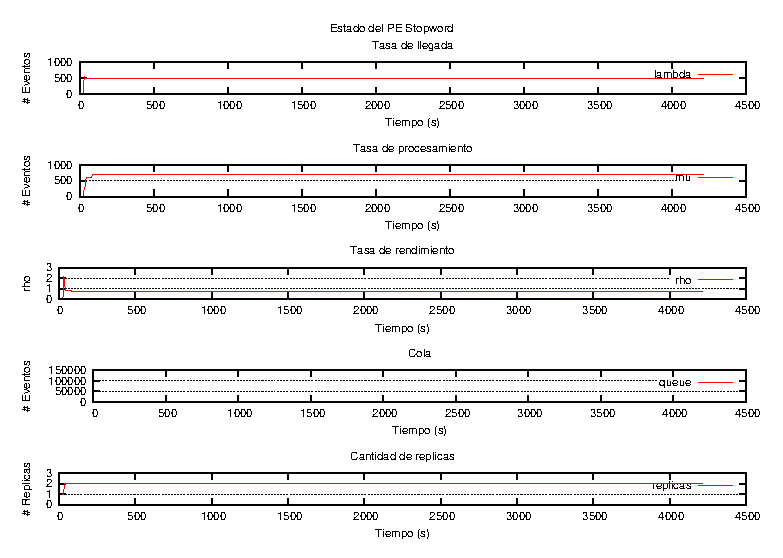
\includegraphics[scale=1.1]{images/exp/app1/uniform/cm/statusStopwordPE.eps}
    \caption{Estadísticas del PE Stopword en la primera aplicación con un envío constante de la fuente de datos con uso del monitor.}
    \label{fig:app1-uniform-statusStopwordPE-cm}
\end{figure}

\begin{figure}[p]
\centering
    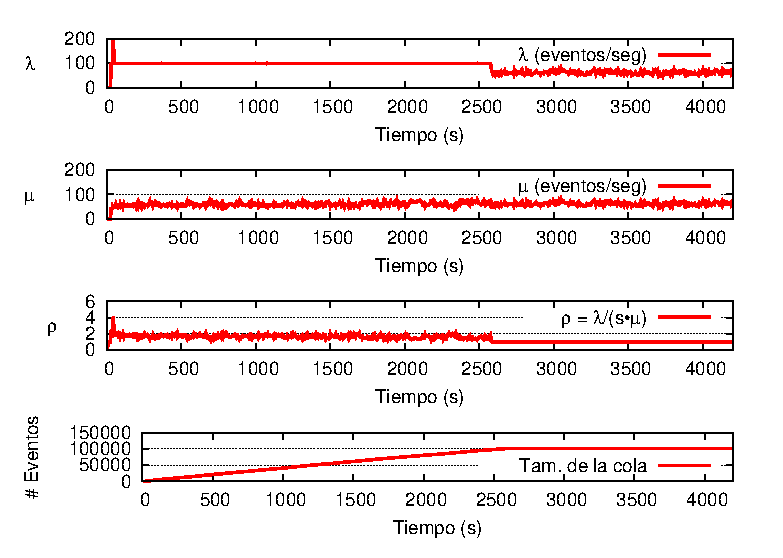
\includegraphics[scale=1.1]{images/exp/app1/uniform/sm/statusStopwordPE.eps}
    \caption{Estadísticas del PE Stopword en la primera aplicación con un envío constante de la fuente de datos sin uso del monitor.}
    \label{fig:app1-uniform-statusStopwordPE-sm}
\end{figure}

\begin{figure}[p]
\centering
    \includegraphics[scale=1.1]{images/exp/app1/uniform/cm/statusLanguagePE.eps}
    \caption{Estadísticas del PE Language en la primera aplicación con un envío constante de la fuente de datos con uso del monitor.}
    \label{fig:app1-uniform-statusLanguagePE-cm}
\end{figure}

\begin{figure}[p]
\centering
    \includegraphics[scale=1.1]{images/exp/app1/uniform/sm/statusLanguagePE.eps}
    \caption{Estadísticas del PE Language en la primera aplicación con un envío constante de la fuente de datos sin uso del monitor.}
    \label{fig:app1-uniform-statusLanguagePE-sm}
\end{figure}

\begin{figure}[p]
\centering
    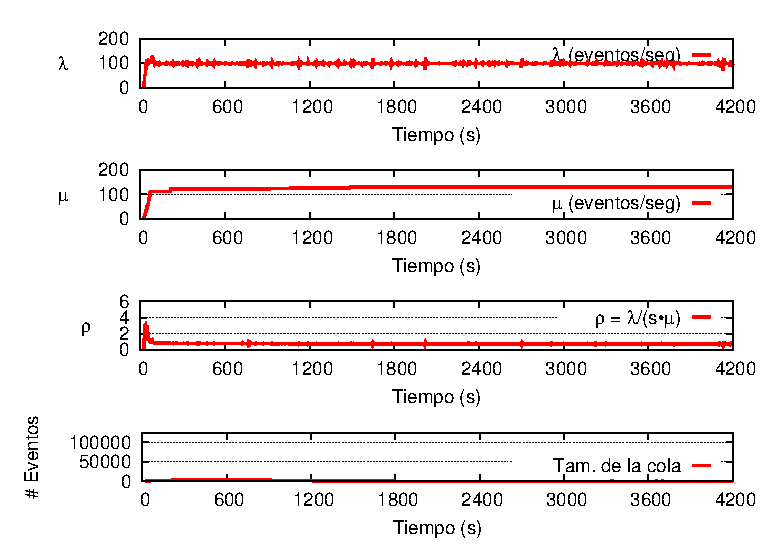
\includegraphics[scale=1.1]{images/exp/app1/uniform/cm/statusCounterPE.eps}
    \caption{Estadísticas del PE Counter en la primera aplicación con un envío constante de la fuente de datos con uso del monitor.}
    \label{fig:app1-uniform-statusCounterPE-cm}
\end{figure}

\begin{figure}[p]
\centering
    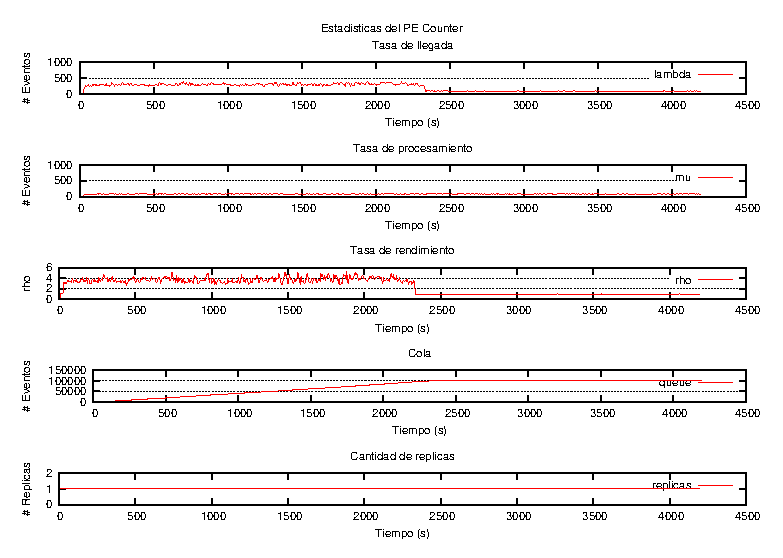
\includegraphics[scale=1.1]{images/exp/app1/uniform/sm/statusCounterPE.eps}
    \caption{Estadísticas del PE Counter en la primera aplicación con un envío constante de la fuente de datos sin uso del monitor.}
    \label{fig:app1-uniform-statusCounterPE-sm}
\end{figure}

\begin{figure}[p]
\centering
    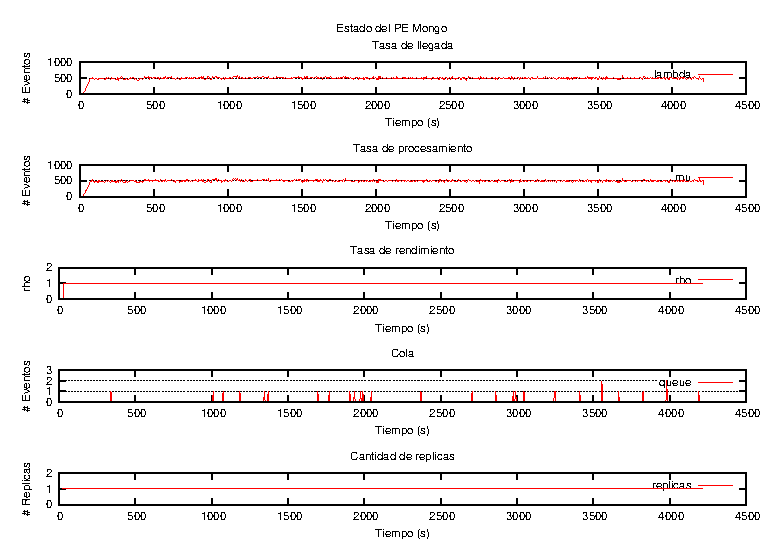
\includegraphics[scale=1.1]{images/exp/app1/uniform/cm/statusMongoPE.eps}
    \caption{Estadísticas del PE Mongo en la primera aplicación con un envío constante de la fuente de datos con uso del monitor.}
    \label{fig:app1-uniform-statusMongoPE-cm}
\end{figure}

\begin{figure}[p]
\centering
    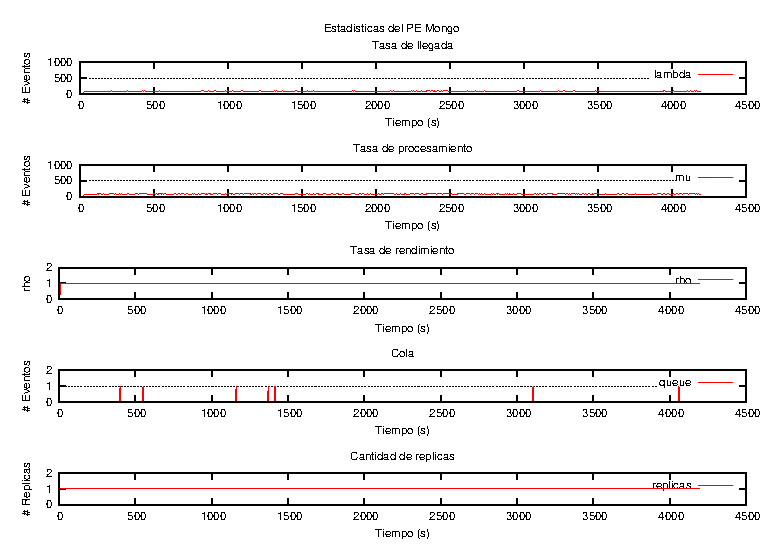
\includegraphics[scale=1.1]{images/exp/app1/uniform/sm/statusMongoPE.eps}
    \caption{Estadísticas del PE Mongo en la primera aplicación con un envío constante de la fuente de datos sin uso del monitor.}
    \label{fig:app1-uniform-statusMongoPE-sm}
\end{figure}

\begin{figure}[ht]
\centering

\begin{minipage}[c]{0.45\textwidth}
\centering
    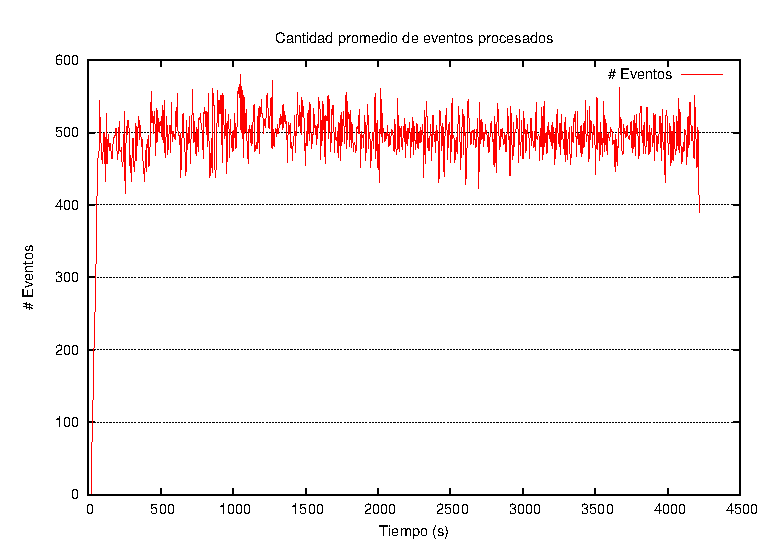
\includegraphics[width=\textwidth]{images/exp/app1/uniform/cm/avgEventProcess.eps}
    \caption{Tiempo promedio de procesamiento de un evento en la primera aplicación con una fuente de datos de distribución uniforme usando monitor.}
    \label{fig:app1-uniform-cm-avgEventProcess}
\end{minipage} \hspace*{1cm}
\begin{minipage}[c]{0.45\textwidth}
\centering
    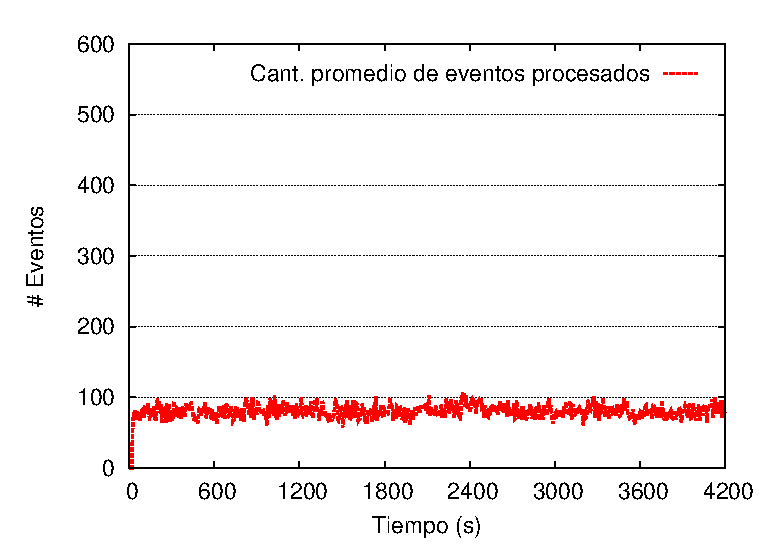
\includegraphics[width=\textwidth]{images/exp/app1/uniform/sm/avgEventProcess.eps}
    \caption{Tiempo promedio de procesamiento de un evento en la primera aplicación con una fuente de datos de distribución uniforme no usando monitor.}
    \label{fig:app1-uniform-sm-avgEventProcess}
\end{minipage}

\end{figure}

\begin{figure}[ht]
\centering

\begin{minipage}[c]{0.45\textwidth}
\centering
    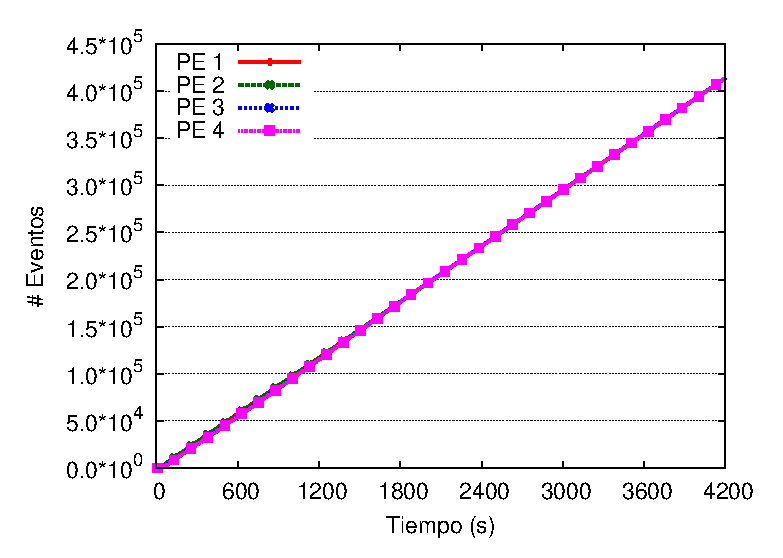
\includegraphics[width=\textwidth]{images/exp/app1/uniform/cm/eventCount.eps}
    \caption{Cantidad total de eventos procesados en la primera aplicación con una fuente de datos de distribución uniforme usando monitor.}
    \label{fig:app1-uniform-eventCount-cm}
\end{minipage} \hspace*{1cm}
\begin{minipage}[c]{0.45\textwidth}
\centering
    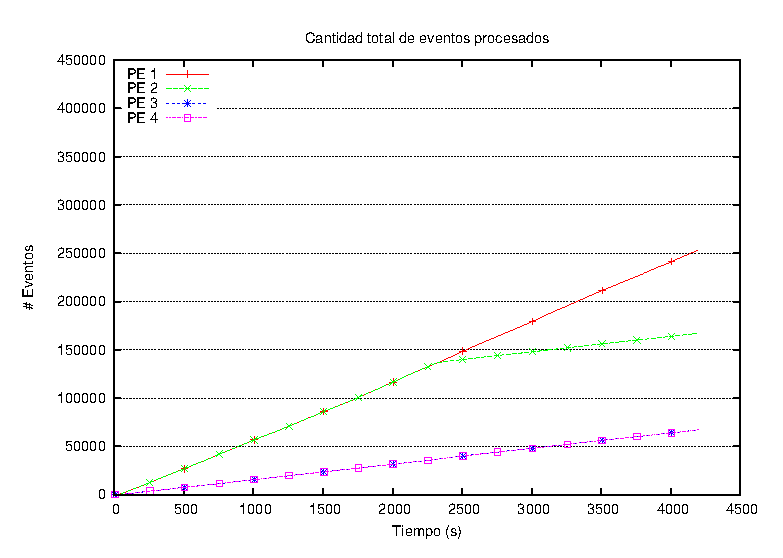
\includegraphics[width=\textwidth]{images/exp/app1/uniform/sm/eventCount.eps}
    \caption{Cantidad total de eventos procesados en la primera aplicación con una fuente de datos de distribución uniforme no usando monitor.}
    \label{fig:app1-uniform-eventCount-sm}
\end{minipage}

\end{figure}

El segundo experimento consistió en enviar un flujo dinámico de datos, y realizando una comparación de los sistemas con y sin monitoreo de la carga de los operadores.

En construcción...

%Para analizar el comportamiento del sistema, se puede observar en la Figura \ref{fig:app1-normal-statusStopwordPE-cm} y \ref{fig:app1-normal-statusStopwordPE-sm} las estadísticas del primer operador del grafo, con y sin monitoreo en la carga de los operadores respectivamente. La tasa de llegada ($\lambda$) se puede observar como en el primer gráfico es dinámica, pero no así en el segundo gráfico, debido que en el segundo 2600 surge una disminución del flujo de datos. Esto se debe a la acumulación de eventos en el \textit{buffer}, por lo que se genera cola en el PE, lo cual impide almacenar mayor cantidad de eventos, dado que la cantidad de eventos que se procesan es menor que la cantidad de eventos que llegan.

%Por otra parte, la tasa de rendimiento de la Figura \ref{fig:app1-normal-statusStopwordPE-cm} se estabiliza dentro de los primeros 100 segundos, debido que el sistema de distribución de carga detectó una sobrecarga en el operador y replicó el operador, a diferencia de la Figura \ref{fig:app1-normal-statusStopwordPE-sm}, en el cual el operador posee una tasa de rendimiento estable que bordea entre 1 y 2, hasta el segundo 2600, donde disminuye debido que la tasa de llegada es menor.

%En la Figura \ref{fig:app1-normal-statusLanguagePE-cm} y \ref{fig:app1-normal-statusLanguagePE-sm} se puede ver el siguiente operador del gráfico, el cual no tiene mayor inconveniente, a excepción del segundo 2400, donde el sin monitoreo disminuye considerablemente la tasa de procesamiento del PE. Si analizamos la Figura \ref{fig:app1-normal-statusStopwordPE-sm} y \ref{fig:app1-normal-statusLanguagePE-sm}, empiezan aproximadamente desde el rango de tiempo (2400s,2600s) los problemas de procesamiento de los operadores, por lo tanto, se puede deducir que si el problema surge en un operador no es un problema aislado, sino que también influye a los siguientes operadores.

%Por otra parte, en la Figura \ref{fig:app1-normal-statusCounterPE-cm}, se puede observar como con el transcurs de los primeros 100 segundos fue aumentando la cantidad de réplicas hasta llegar a 5, el cual fue su óptimo, para ir procesando la cantidad de eventos y disminuir la cola existente en el sistema. Esto en contra posición a la Figura \ref{fig:app1-normal-statusCounterPE-sm}, donde la inexistencia de replicación, genera una cola la cual se mantiene constante en el segundo 2400. Esto se debe a que la cantidad de eventos almacenados en el \textit{buffer} está lleno, por lo que no pueden agregarse más eventos y bloqueando el \textit{buffer}.

%Finalmente, se encuentra el último operador, el cual no presenta grandes inconvenientes tanto en la Figura \ref{fig:app1-normal-statusMongoPE-cm} y \ref{fig:app1-normal-statusMongoPE-sm}, esto debido que el tiempo de procesamiento es bajo, y nunca llega una cantidad de eventos considerable para existir una sobrecarga en éste. Además es importante destacar que en la Figura \ref{fig:app1-normal-statusMongoPE-sm} llega una menor tasa de llegada, exactamente un $83,827\%$ menos de eventos que un SPS ejecutado con el sistema de distribución de carga.

%Por otra parte, también se analizó la cantidad promedio de eventos procesados en cada período, la cual está graficada en la Figura \ref{fig:app1-normal-avgEventProcess}. Como se puede apreciar, en los primeros 50 segundos se puede ver una mejora considerable en la cantidad de eventos procesados, donde posteriormente se procesan aproximadamente 480 eventos por período con monitoreo, a diferencia del SPS sin monitoreo, que procesa 90 eventos por período aproximadamente, habiendo una mejora del $615,38\%$. Esta mejora se debe al factor de la replicación de los operadores que posee mayor sobrecarga, por lo que al aumentar la cantidad de réplicas, aumenta la tasa de procesamiento, lo significa mayor cantidad de flujo para el próximo operador.

%Así también, se puede observar en la Figura \ref{fig:app1-normal-eventCount-cm} y \ref{fig:app1-normal-eventCount-sm} la cantidad total de eventos procesados con el transcurso de la ejecución en cada uno de los operadores, con y sin uso del monitoreo respectivamente. En el primer gráfico se denota como los cuatro operadores del SPS van aumentando casi linealmente de la misma manera, tan sólo existe una menor cantidad de eventos procesados en el tercer PE, lo cual se traslada al cuatro PE, debido que al procesar menor cantidad de eventos el tercer PE, llega menor cantidad de datos al cuarto PE. En este gráfico se llegó a un total de 401.618 eventos procesados. En cambio, en el segundo gráfico existe una curva muy distinta por los distintos operadores, lo cual se ve reflejado desde la cantidad de eventos procesados en el primer operador hasta la cantidad total de eventos procesados por el sistema, el cual es de 67.141, existiendo una mejora del $598,171\%$ con el uso del sistema de distribución de carga.

%\begin{figure}[p]
%\centering
%    \includegraphics[scale=1.1.1]{images/exp/app1/normal/cm/statusStopwordPE.eps}
%    \caption{Estadísticas del PE Stopword en la primera aplicación con un envío constante de la fuente de datos con uso del monitor.}
%    \label{fig:app1-uniform-statusStopwordPE-cm}
%\end{figure}
%
%\begin{figure}[p]
%\centering
%    \includegraphics[scale=1.1.1]{images/exp/app1/normal/sm/statusStopwordPE.eps}
%    \caption{Estadísticas del PE Stopword en la primera aplicación con un envío constante de la fuente de datos sin uso del monitor.}
%    \label{fig:app1-uniform-statusStopwordPE-sm}
%\end{figure}
%
%\begin{figure}[p]
%\centering
%    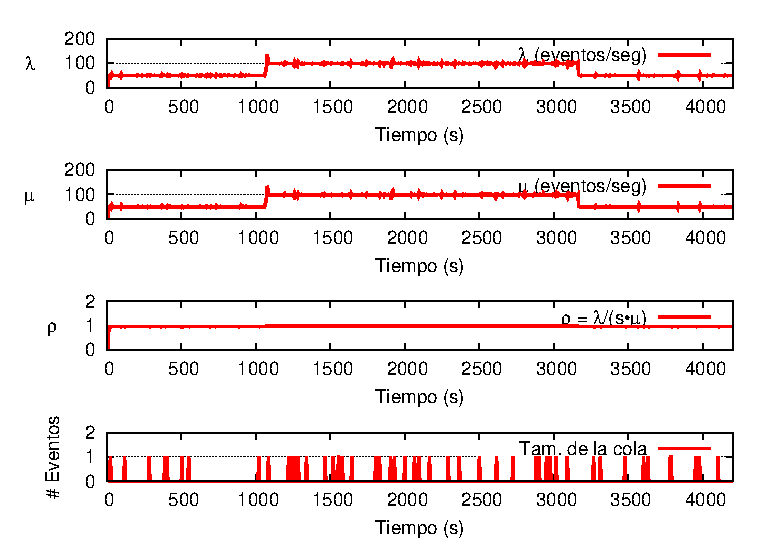
\includegraphics[scale=1.1]{images/exp/app1/normal/cm/statusLanguagePE.eps}
%    \caption{Estadísticas del PE Language en la primera aplicación con un envío constante de la fuente de datos con uso del monitor.}
%    \label{fig:app1-uniform-statusLanguagePE-cm}
%\end{figure}
%
%\begin{figure}[p]
%\centering
%    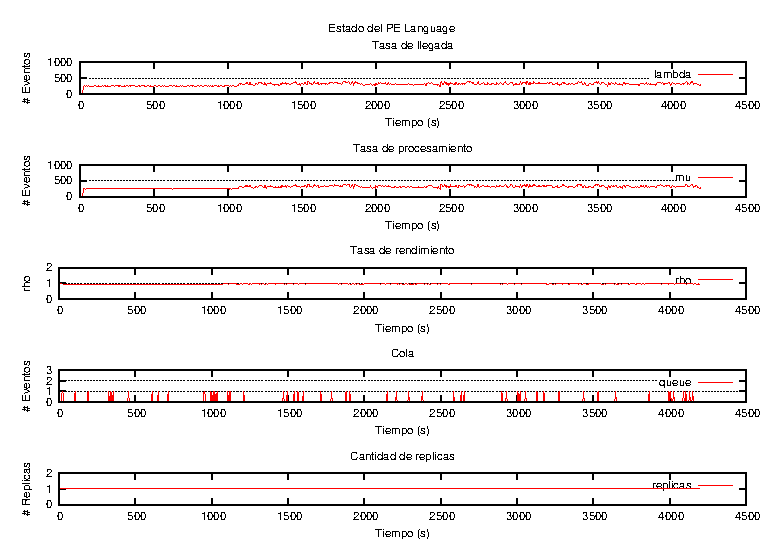
\includegraphics[scale=1.1]{images/exp/app1/normal/sm/statusLanguagePE.eps}
%    \caption{Estadísticas del PE Language en la primera aplicación con un envío constante de la fuente de datos sin uso del monitor.}
%    \label{fig:app1-uniform-statusLanguagePE-sm}
%\end{figure}
%
%\begin{figure}[p]
%\centering
%    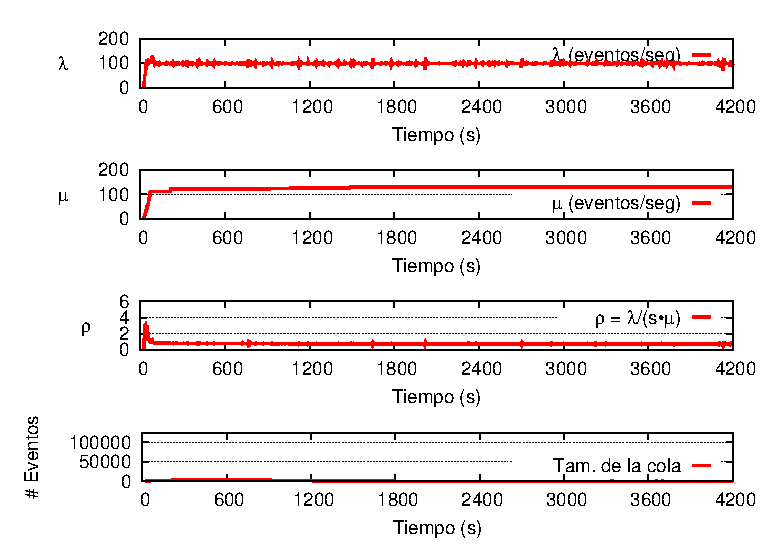
\includegraphics[scale=1.1]{images/exp/app1/uniform/cm/statusCounterPE.eps}
%    \caption{Estadísticas del PE Counter en la primera aplicación con un envío constante de la fuente de datos con uso del monitor.}
%    \label{fig:app1-uniform-statusCounterPE-cm}
%\end{figure}
%
%\begin{figure}[p]
%\centering
%    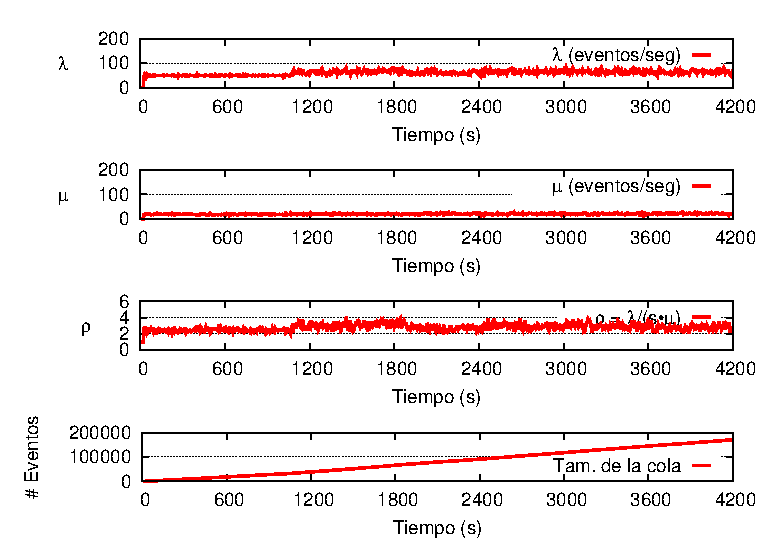
\includegraphics[scale=1.1]{images/exp/app1/normal/sm/statusCounterPE.eps}
%    \caption{Estadísticas del PE Counter en la primera aplicación con un envío constante de la fuente de datos sin uso del monitor.}
%    \label{fig:app1-uniform-statusCounterPE-sm}
%\end{figure}
%
%\begin{figure}[p]
%\centering
%    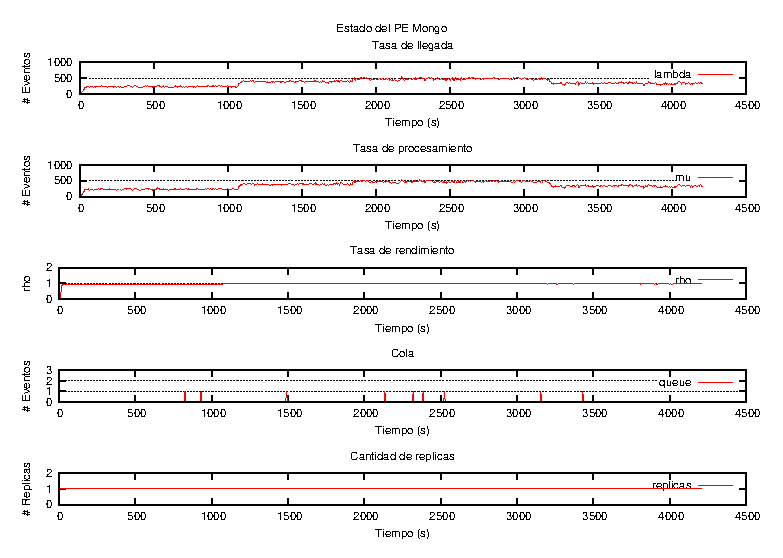
\includegraphics[scale=1.1]{images/exp/app1/normal/cm/statusMongoPE.eps}
%    \caption{Estadísticas del PE Mongo en la primera aplicación con un envío constante de la fuente de datos con uso del monitor.}
%    \label{fig:app1-uniform-statusMongoPE-cm}
%\end{figure}
%
%\begin{figure}[p]
%\centering
%    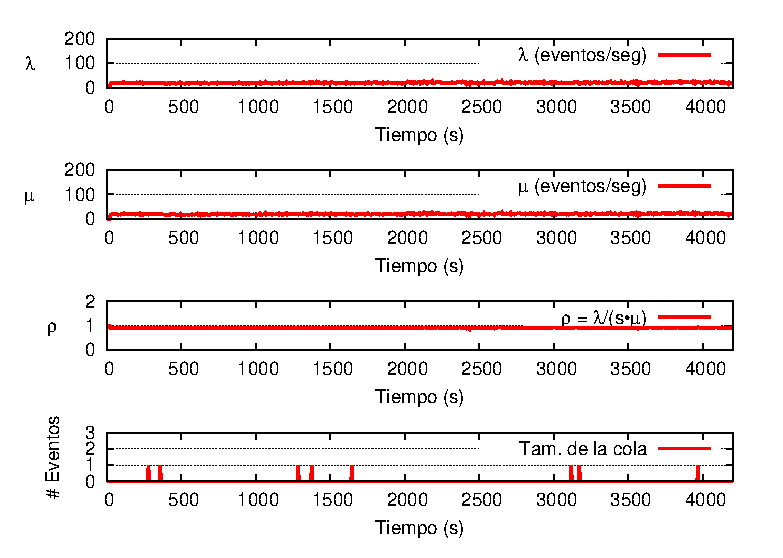
\includegraphics[scale=1.1]{images/exp/app1/normal/sm/statusMongoPE.eps}
%    \caption{Estadísticas del PE Mongo en la primera aplicación con un envío constante de la fuente de datos sin uso del monitor.}
%    \label{fig:app1-uniform-statusMongoPE-sm}
%\end{figure}
%
%\begin{figure}[ht]
%\centering
%
%\begin{minipage}[c]{0.45\textwidth}
%\centering
%    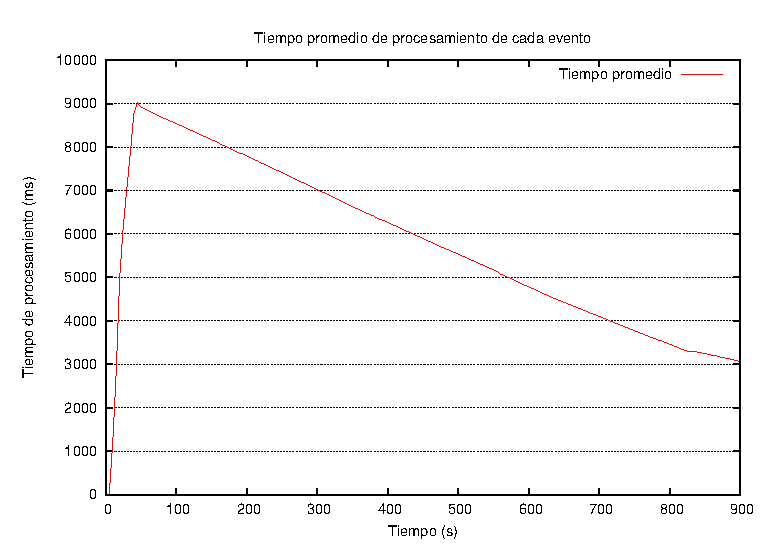
\includegraphics[width=\textwidth]{images/exp/app1/normal/avgTimeTotal.eps}
%    \caption{Tiempo promedio de procesamiento de un evento en la primera aplicación con una fuente de datos de distribución uniforme.}
%    \label{fig:app1-uniform-avgTimeTotal}
%\end{minipage} \hspace*{1cm}
%\begin{minipage}[c]{0.45\textwidth}
%\centering
%    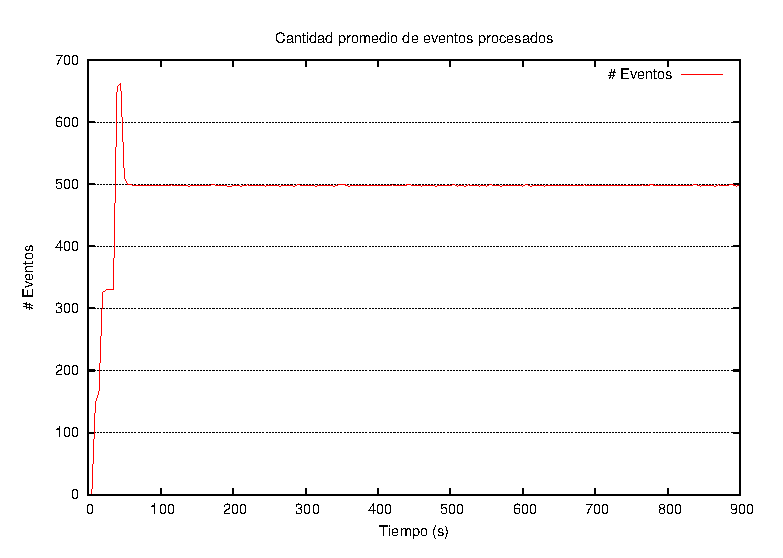
\includegraphics[width=\textwidth]{images/exp/app1/normal/avgEventProcess.eps}
%    \caption{Cantidad promedio de eventos procesados en un período de tiempo en la primera aplicación con una fuente de datos de distribución uniforme.}
%    \label{fig:app1-uniform-avgEventProcess}
%\end{minipage}
%
%\end{figure}
%
%\begin{figure}[ht]
%\centering
%
%\begin{minipage}[c]{0.45\textwidth}
%\centering
%    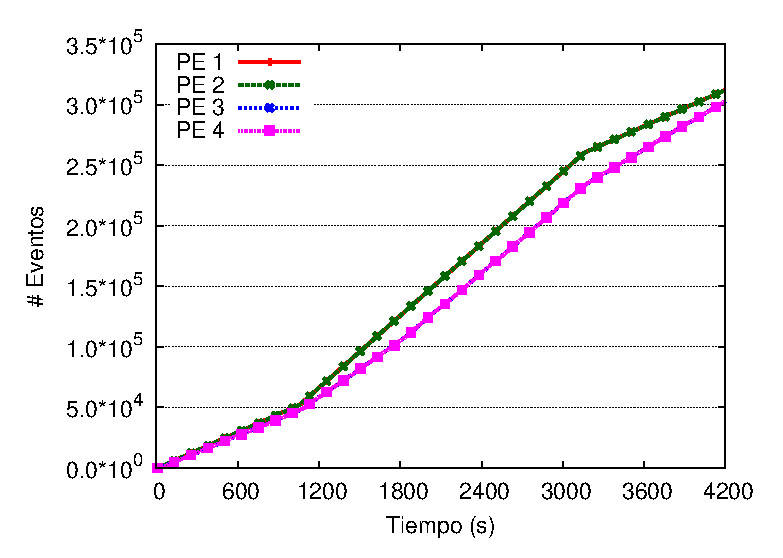
\includegraphics[width=\textwidth]{images/exp/app1/normal/cm/eventCount.eps}
%    \caption{Cantidad total de eventos procesados en la primera aplicación con una fuente de datos de distribución uniforme usando monitor.}
%    \label{fig:app1-uniform-eventCount-cm}
%\end{minipage} \hspace*{1cm}
%\begin{minipage}[c]{0.45\textwidth}
%\centering
%    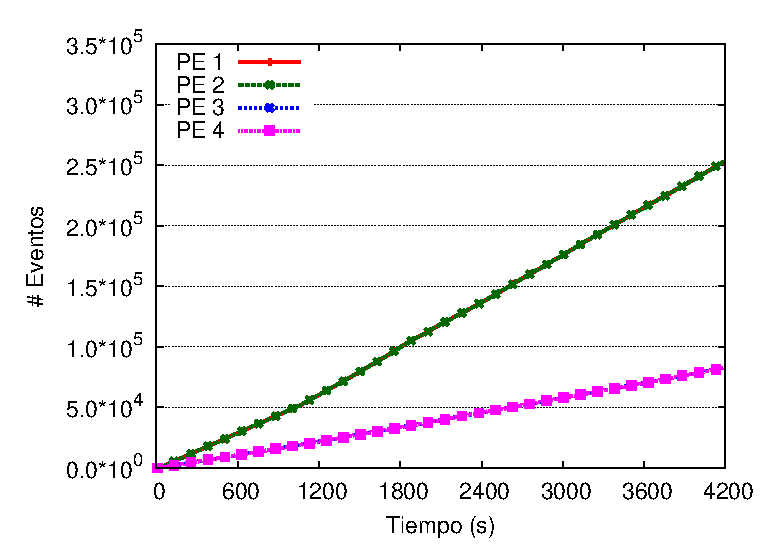
\includegraphics[width=\textwidth]{images/exp/app1/normal/sm/eventCount.eps}
%    \caption{Cantidad total de eventos procesados en la primera aplicación con una fuente de datos de distribución uniforme no usando monitor.}
%    \label{fig:app1-uniform-eventCount-sm}
%\end{minipage}
%
%\end{figure}

\subsection{Segundo experimento}
En la segunda aplicación se procedió a realizar cuatro experimentos distintos, donde cada par era una comparación del experimento con y sin uso del monitor. Las dos primeras se consideró un envío constante de la fuente de datos, y las dos segundas se consideró un envío dinámico de la fuente de datos.

Para el análisis de los experimento se consideró la cantidad total de eventos y las estadísticas de cada PE en el transcurso de la ejecución de la aplicación.

Para analizar el comportamiento del sistema, se puede observar en la Figura \ref{fig:app2-uniform-statusSplitPE-cm} y \ref{fig:app2-uniform-statusSplitPE-sm} las estadísticas del primer operador del grafo, con y sin monitoreo en la carga de los operadores respectivamente. En el primer gráfico la tasa de llegada ($\lambda$) en los primeros 200 segundos se encuentran ciertos \textit{peak}, los cuales se deben al \textit{delay} en la toma de estadísticas, producto de la replicación del siguiente PE en el sistema, como se puede demostrar en la Figura \ref{fig:app2-uniform-statusCounterPE-cm}. Independiente del uso del monitoreo, se puede denotar que el comportamiento entre los dos PEs es prácticamente igual, y esto se debe a que la carga que posee este PE es casi nula, debido que es un PE auxiliar para el PE Counter, dado que sólo separa la cantidad de palabras para que el PE Counter cuente la frecuencia de cada palabra en la información entrante.

En cambio, en la Figura \ref{fig:app2-uniform-statusCounterPE-cm} y \ref{fig:app2-uniform-statusCounterPE-sm} se puede observar una diferencia en los rendimientos del PE. Esto se debe, a que este operador posee una carga una alta carga, dado que posee una gran bolsa de palabras para comparar con las palabras del \textit{tweets}. Debido a esto, al generar las réplicas, se produce una mejora considerable del operador en los primeros 100 segundo.

En este caso, el predictor se activó, dado que se realiza un aumento de 9 a 14 réplicas. Si bien, la cantidad de réplicas fue mayor a lo necesario, dado que el promedio de tasa de procesamiento posterior al segundo 100 es de 0.63, no se considera el operador en estado ocioso, por lo que no se disminuye la cantidad de réplicas.

Un detalle importante a destacar, es que independiente que se generen más réplicas, el sistema no procesa mayor cantidad de eventos, como se puede observar en la cola del operador. Este problema fue detectado por la implementanción realizada en el SPS de S4, dado que posterior a un período de tiempo, la tasa de procesamiento disminuye considerablemente. La hipótesis que se posee de este problema es que el sistema no elimina los eventos procesados, por lo que independiente de si es procesado o no, continúa en el \textit{buffer}, de esta manera, la cola sigue aumentando, sin ser removido por el \textit{garbage collector} de Java.

En el último PE, se puede ver que existe una baja cantidad de eventos entrantes, como se muestra en la Figura \ref{fig:app2-uniform-statusMergePE-cm} y \ref{fig:app2-uniform-statusMergePE-sm}. Esto se debe, a que los eventos entrantes sólo son enviados cada 10 segundos por el PE Counter, por lo que son una pequeña cantidad de eventos los que son enviados. En el primer gráfico, se puede ver que la tasa de llegada aumenta posterior a los 100 segundos, esto se debe a que se realizaron réplicas, por lo que cada una de las réplicas envía un evento cada 10 segundos, habiendo mayor flujo. En cambio, en el segundo gráfico, el flujo de entrada sólo se condiciona por una réplica, por lo que no se procesa la misma cantidad de eventos. Cabe destacar, que como la tasa de llegada es pequeña, no existe un problema en la tasa de rendimiento del operador, aunque posea un alto cómputo de ejecución su tarea.

Finalmente, en la Figura \ref{fig:app2-uniform-eventCount-cm} y \ref{fig:app2-uniform-eventCount-sm} se muestra la cantidad total de eventos procesados. En el primer gráfico se puede analizar que la diferencia de la pendiente entre las rectas del primer y segundo PE, es menor que en el segundo gráfico. Esto se debe al aumento de la cantidad de réplicas, de esta manera puede procesar mayor cantidad de eventos, siendo un procesamiento de 181114 con uso el monitor contra 30049 sin uso del monitor, habiendo una mejora del $602,7288\%$. El tercer PE procesa pocos eventos, debido que sólo le llega un evento por réplica cada 10 segundos.

Dentro de los análisis importantes a realizar por parte de este experimento, es que en el gráfico \ref{fig:app1-uniform-eventCount-cm} no existe una mejora por parte del segundo PE de manera paralela al flujo de datos emanado por el primer PE. Esto se debió al funcionamiento de la herramienta S4, debido que después de un período de tiempo no procesa la misma cantidad de eventos, por lo que independiente que se siga replicando, no existe una mejora en el sistema. Este problema se debe a la forma en que esta implementando el \textit{buffer} de S4, debido que éste se va llenando, pero no se libera, por lo que al llenarse bloquea el envió de los datos por parte del sistema, generando una demora en el procesamiento.

\begin{figure}[p]
\centering
    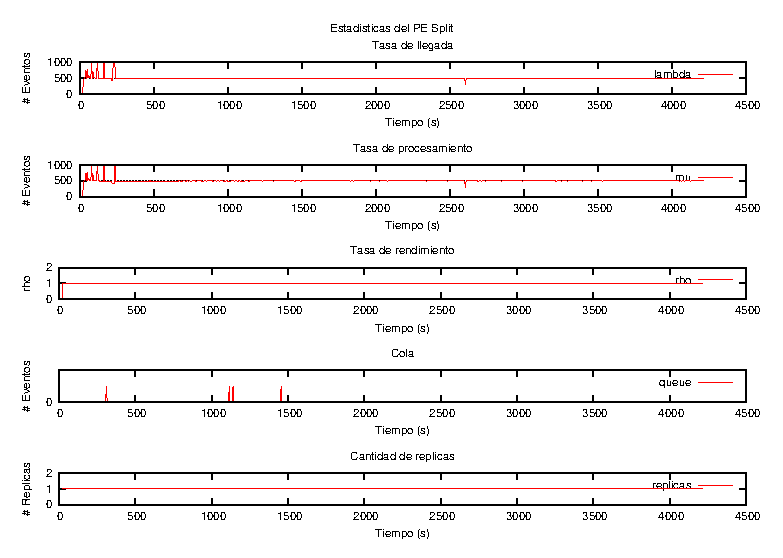
\includegraphics[scale=1.1]{images/exp/app2/uniform/cm/statusSplitPE.eps}
    \caption{Estadísticas del PE Mongo en la primera aplicación con un envío constante de la fuente de datos con uso del monitor.}
    \label{fig:app2-uniform-statusSplitPE-cm}
\end{figure}

\begin{figure}[p]
\centering
    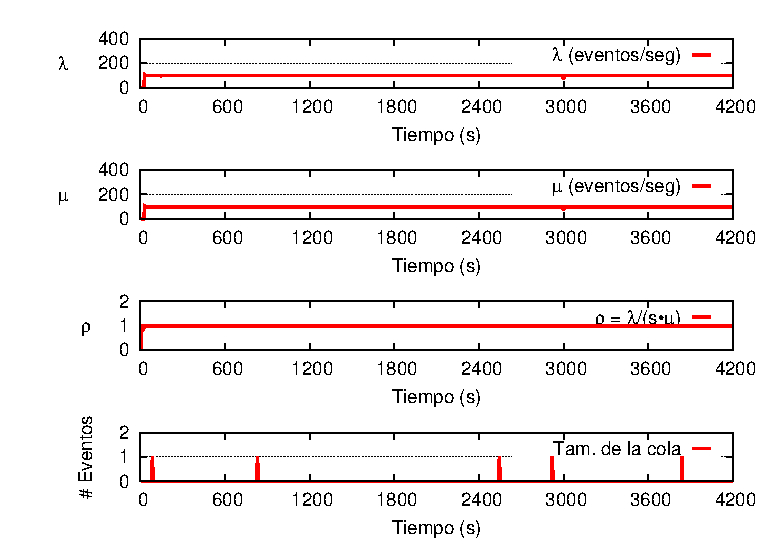
\includegraphics[scale=1.1]{images/exp/app2/uniform/sm/statusSplitPE.eps}
    \caption{Estadísticas del PE Mongo en la primera aplicación con un envío constante de la fuente de datos sin uso del monitor.}
    \label{fig:app2-uniform-statusSplitPE-sm}
\end{figure}

\begin{figure}[p]
\centering
    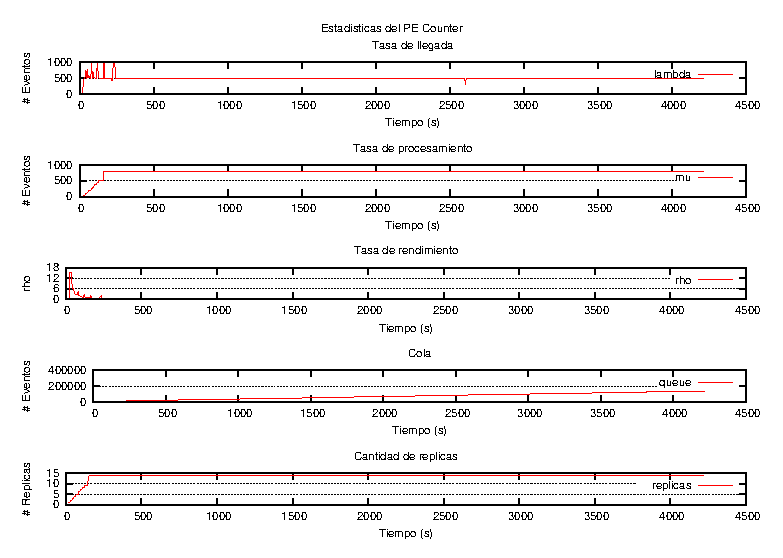
\includegraphics[scale=1.1]{images/exp/app2/uniform/cm/statusCounterPE.eps}
    \caption{Estadísticas del PE Mongo en la primera aplicación con un envío constante de la fuente de datos con uso del monitor.}
    \label{fig:app2-uniform-statusCounterPE-cm}
\end{figure}

\begin{figure}[p]
\centering
    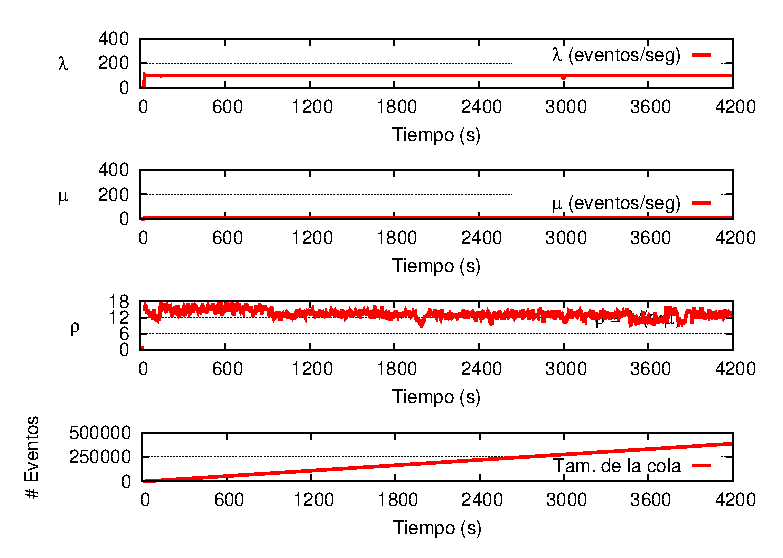
\includegraphics[scale=1.1]{images/exp/app2/uniform/sm/statusCounterPE.eps}
    \caption{Estadísticas del PE Mongo en la primera aplicación con un envío constante de la fuente de datos sin uso del monitor.}
    \label{fig:app2-uniform-statusCounterPE-sm}
\end{figure}

\begin{figure}[p]
\centering
    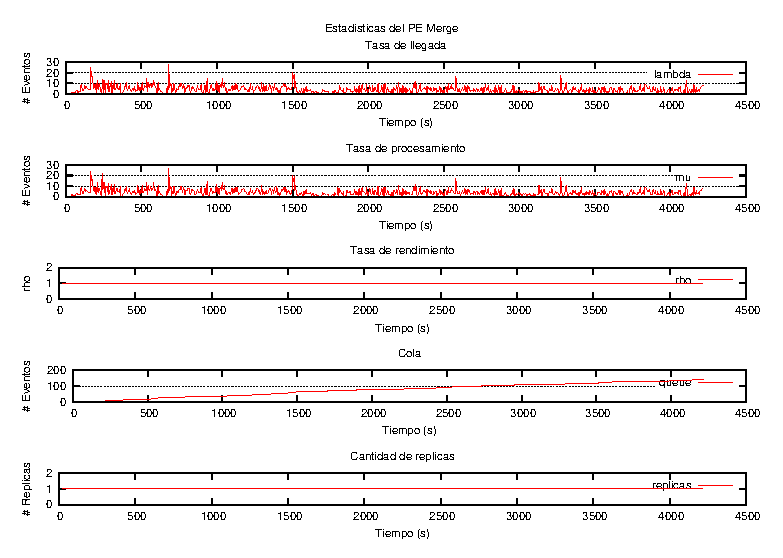
\includegraphics[scale=1.1]{images/exp/app2/uniform/cm/statusMergePE.eps}
    \caption{Estadísticas del PE Mongo en la primera aplicación con un envío constante de la fuente de datos con uso del monitor.}
    \label{fig:app2-uniform-statusMergePE-cm}
\end{figure}

\begin{figure}[p]
\centering
    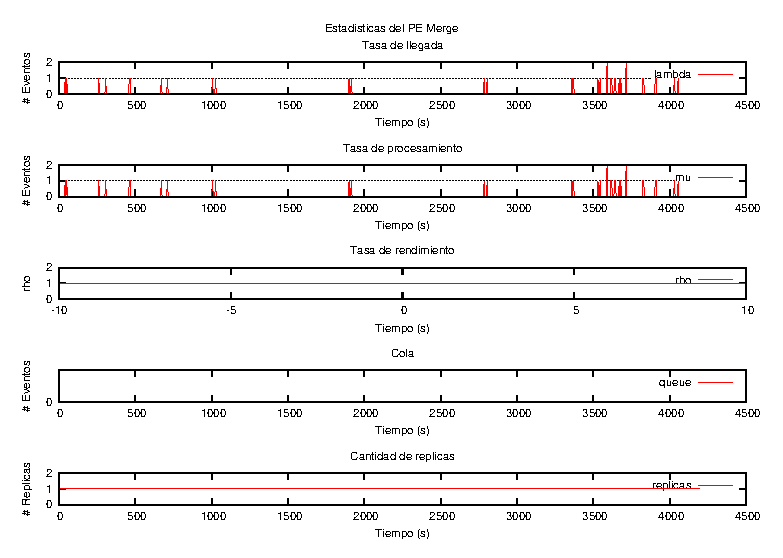
\includegraphics[scale=1.1]{images/exp/app2/uniform/sm/statusMergePE.eps}
    \caption{Estadísticas del PE Mongo en la primera aplicación con un envío constante de la fuente de datos sin uso del monitor.}
    \label{fig:app2-uniform-statusMergePE-sm}
\end{figure}

\begin{figure}[ht]
\centering

\begin{minipage}[c]{0.45\textwidth}
\centering
    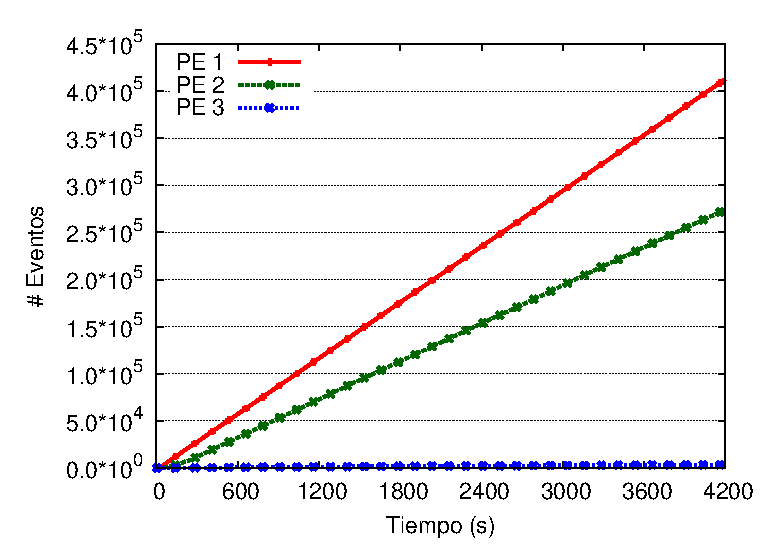
\includegraphics[width=\textwidth]{images/exp/app2/uniform/cm/eventCount.eps}
    \caption{Cantidad total de eventos procesados en la primera aplicación con una fuente de datos de distribución uniforme usando monitor.}
    \label{fig:app2-uniform-eventCount-cm}
\end{minipage} \hspace*{1cm}
\begin{minipage}[c]{0.45\textwidth}
\centering
    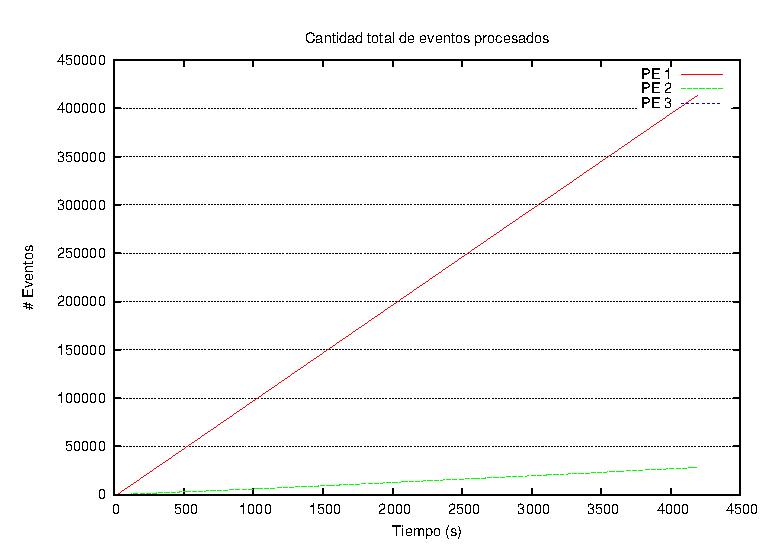
\includegraphics[width=\textwidth]{images/exp/app2/uniform/sm/eventCount.eps}
    \caption{Cantidad total de eventos procesados en la primera aplicación con una fuente de datos de distribución uniforme no usando monitor.}
    \label{fig:app2-uniform-eventCount-sm}
\end{minipage}

\end{figure}

\subsection{Tercer experimento}
En la tercera aplicación se procedió a realizar dos experimentos, ambos con envío constante de la fuente de datos, donde el SPS funciona con y sin uso del monitor.

Para el análisis de los experimento se consideró el consumo de RAM, el uso de la CPU, la cantidad total de eventos, la cantidad promedio de eventos procesados por período y las estadísticas de cada PE en el transcurso de la ejecución de la aplicación.

\begin{figure}[p]
\centering
    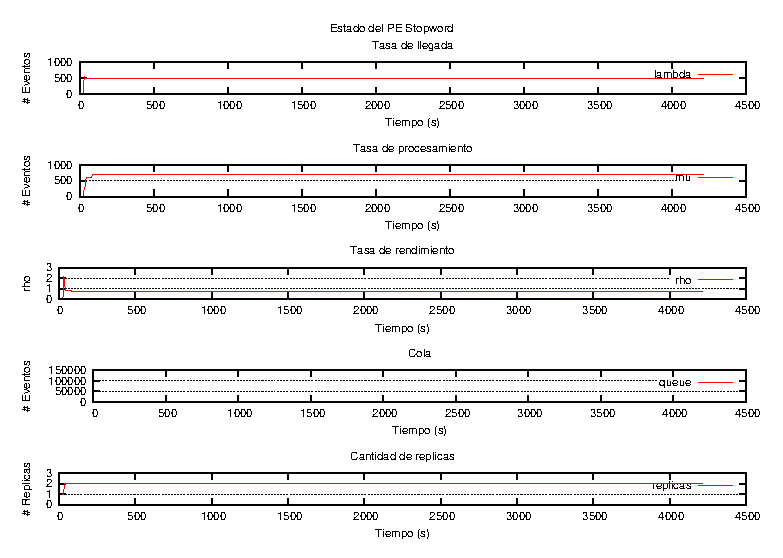
\includegraphics[scale=1.1]{images/exp/app1/uniform/cm/statusStopwordPE.eps}
    \caption{Estadísticas del PE Stopword en la primera aplicación con un envío constante de la fuente de datos con uso del monitor.}
    \label{fig:app1-uniform-statusStopwordPE-cm}
\end{figure}

\begin{figure}[p]
\centering
    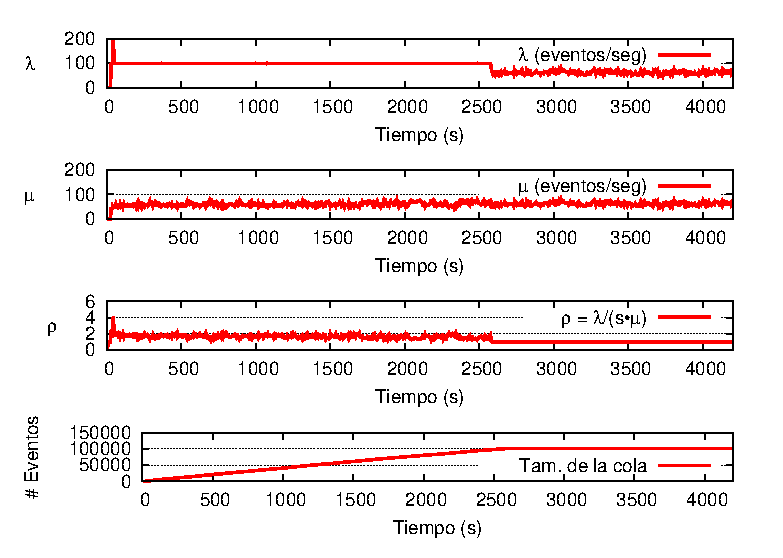
\includegraphics[scale=1.1]{images/exp/app1/uniform/sm/statusStopwordPE.eps}
    \caption{Estadísticas del PE Stopword en la primera aplicación con un envío constante de la fuente de datos sin uso del monitor.}
    \label{fig:app1-uniform-statusStopwordPE-sm}
\end{figure}

\begin{figure}[p]
\centering
    \includegraphics[scale=1.1]{images/exp/app1/uniform/cm/statusLanguagePE.eps}
    \caption{Estadísticas del PE Language en la primera aplicación con un envío constante de la fuente de datos con uso del monitor.}
    \label{fig:app1-uniform-statusLanguagePE-cm}
\end{figure}

\begin{figure}[p]
\centering
    \includegraphics[scale=1.1]{images/exp/app1/uniform/sm/statusLanguagePE.eps}
    \caption{Estadísticas del PE Language en la primera aplicación con un envío constante de la fuente de datos sin uso del monitor.}
    \label{fig:app1-uniform-statusLanguagePE-sm}
\end{figure}

\begin{figure}[p]
\centering
    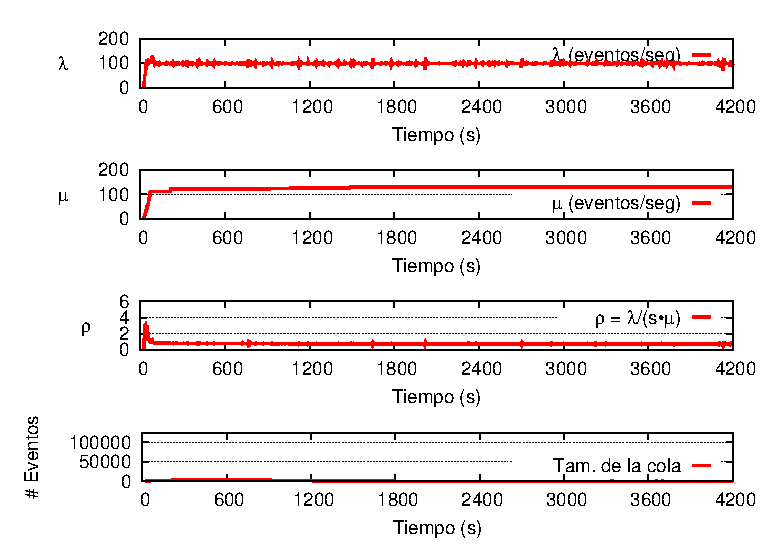
\includegraphics[scale=1.1]{images/exp/app1/uniform/cm/statusCounterPE.eps}
    \caption{Estadísticas del PE Counter en la primera aplicación con un envío constante de la fuente de datos con uso del monitor.}
    \label{fig:app1-uniform-statusCounterPE-cm}
\end{figure}

\begin{figure}[p]
\centering
    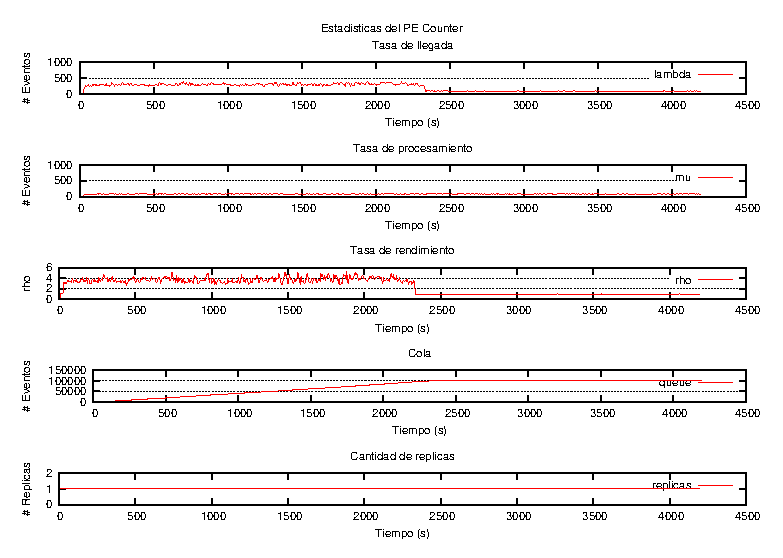
\includegraphics[scale=1.1]{images/exp/app1/uniform/sm/statusCounterPE.eps}
    \caption{Estadísticas del PE Counter en la primera aplicación con un envío constante de la fuente de datos sin uso del monitor.}
    \label{fig:app1-uniform-statusCounterPE-sm}
\end{figure}

\begin{figure}[p]
\centering
    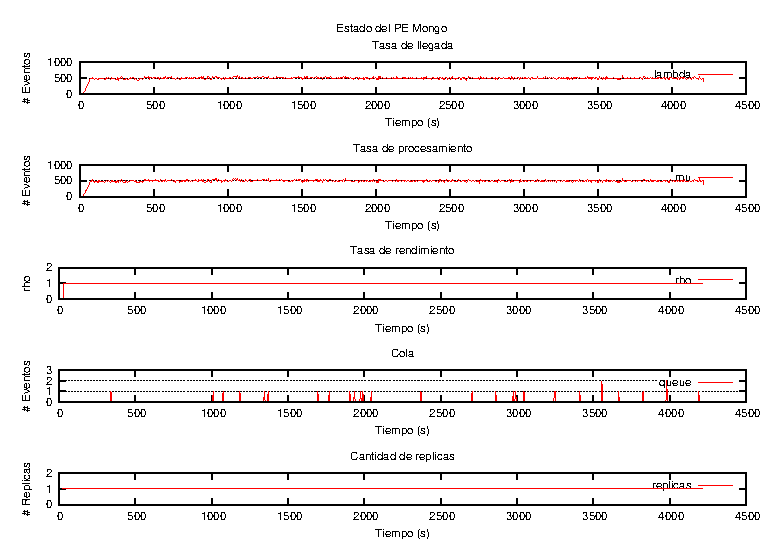
\includegraphics[scale=1.1]{images/exp/app1/uniform/cm/statusMongoPE.eps}
    \caption{Estadísticas del PE Mongo en la primera aplicación con un envío constante de la fuente de datos con uso del monitor.}
    \label{fig:app1-uniform-statusMongoPE-cm}
\end{figure}

\begin{figure}[p]
\centering
    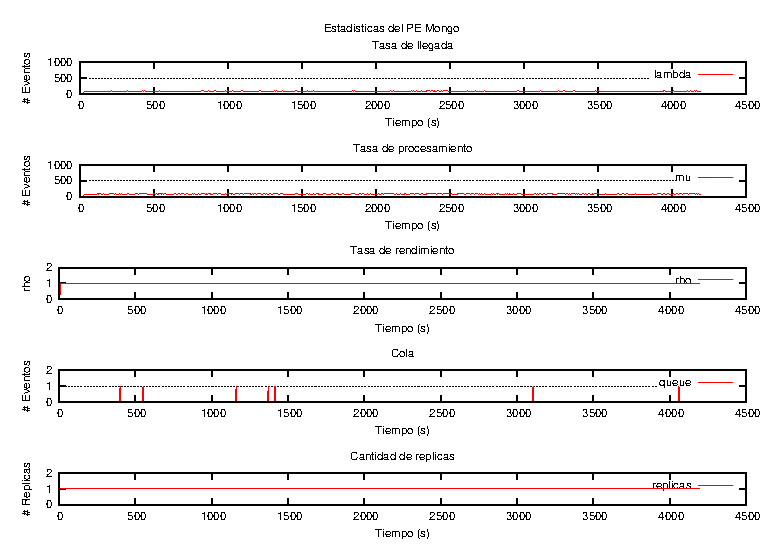
\includegraphics[scale=1.1]{images/exp/app1/uniform/sm/statusMongoPE.eps}
    \caption{Estadísticas del PE Mongo en la primera aplicación con un envío constante de la fuente de datos sin uso del monitor.}
    \label{fig:app1-uniform-statusMongoPE-sm}
\end{figure}

\begin{figure}[ht]
\centering

\begin{minipage}[c]{0.45\textwidth}
\centering
    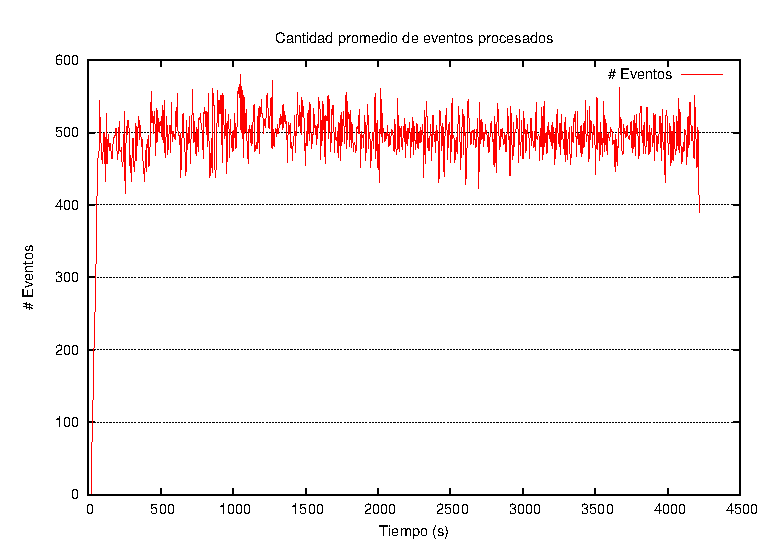
\includegraphics[width=\textwidth]{images/exp/app1/uniform/cm/avgEventProcess.eps}
    \caption{Tiempo promedio de procesamiento de un evento en la primera aplicación con una fuente de datos de distribución uniforme usando monitor.}
    \label{fig:app1-uniform-cm-avgEventProcess}
\end{minipage} \hspace*{1cm}
\begin{minipage}[c]{0.45\textwidth}
\centering
    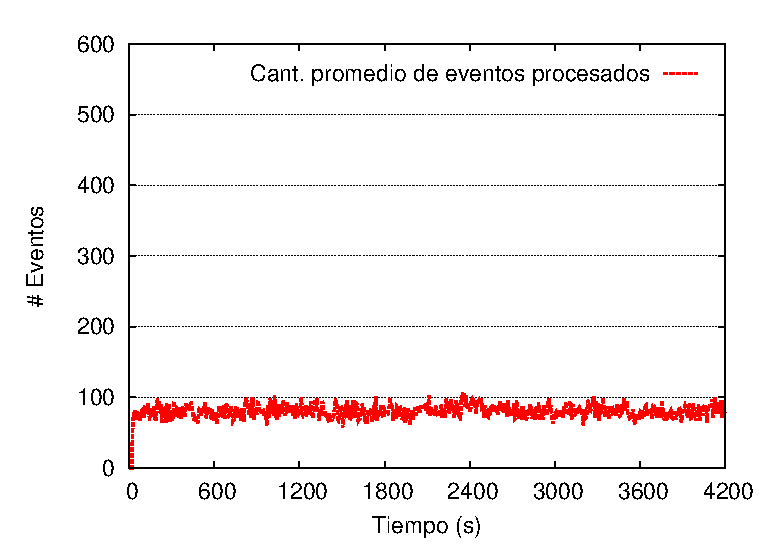
\includegraphics[width=\textwidth]{images/exp/app1/uniform/sm/avgEventProcess.eps}
    \caption{Tiempo promedio de procesamiento de un evento en la primera aplicación con una fuente de datos de distribución uniforme no usando monitor.}
    \label{fig:app1-uniform-sm-avgEventProcess}
\end{minipage}

\end{figure}

\begin{figure}[ht]
\centering

\begin{minipage}[c]{0.45\textwidth}
\centering
    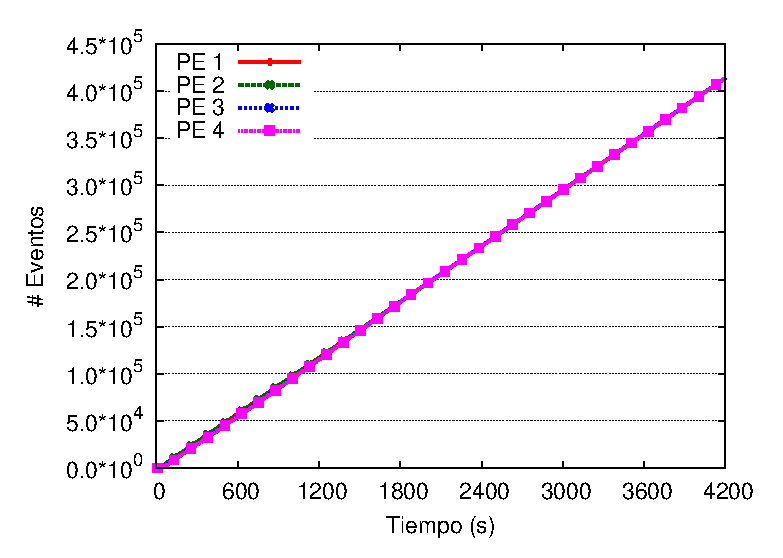
\includegraphics[width=\textwidth]{images/exp/app1/uniform/cm/eventCount.eps}
    \caption{Cantidad total de eventos procesados en la primera aplicación con una fuente de datos de distribución uniforme usando monitor.}
    \label{fig:app1-uniform-eventCount-cm}
\end{minipage} \hspace*{1cm}
\begin{minipage}[c]{0.45\textwidth}
\centering
    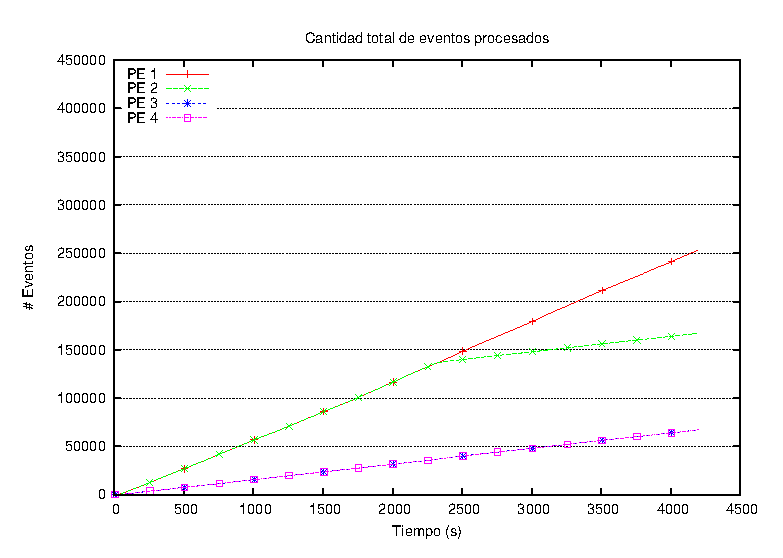
\includegraphics[width=\textwidth]{images/exp/app1/uniform/sm/eventCount.eps}
    \caption{Cantidad total de eventos procesados en la primera aplicación con una fuente de datos de distribución uniforme no usando monitor.}
    \label{fig:app1-uniform-eventCount-sm}
\end{minipage}

\end{figure}